% ============================================================
% Projective Dynamic Logo (PDL)
% Global Mapping of Structures, Results, and Open Problems
% Version 24 — C. Laubscher
% ============================================================
\documentclass[11pt,a4paper]{article}

% ---- Encoding and fonts ----
\usepackage[utf8]{inputenc}
\usepackage[T1]{fontenc}
\usepackage{lmodern}
\usepackage{newtxtext}

% ---- Page layout ----
\usepackage[margin=2.5cm]{geometry}

% ---- Mathematics ----
\usepackage{amsmath,amssymb,amsthm}
\newtheorem{resolvedproblem}{Resolved Problem}
\newcommand{\Rval}{R_{\mathrm{val}}}

% ---- Tables and lists ----
\usepackage{booktabs}
\usepackage{longtable}
\usepackage{array}
\usepackage{ragged2e}
\usepackage{enumitem}
\newcommand{\hb}{\hbar}
\newcommand{\Cspin}{{\mathcal{C}_{\mathrm{spin}}}}
\newcommand{\Cmass}{{\mathcal{C}_{\mathrm{mass}}}}
\newcolumntype{L}[1]{>{\RaggedRight\arraybackslash}p{#1}}

% ---- Graphics ----
\usepackage{graphicx}
\usepackage{float}
\usepackage{tikz}
\usetikzlibrary{positioning,backgrounds,arrows.meta,fit}
\pgfdeclarelayer{background}
\pgfsetlayers{background,main}

% ---- Captions and colours ----
\usepackage[font=small,labelfont=bf]{caption}
\captionsetup[table]{labelsep=quad}
\usepackage{xcolor}
\definecolor{proofblue}{RGB}{0,70,140}
\definecolor{conjecturegreen}{RGB}{0,120,60}
\definecolor{hypothesisorange}{RGB}{200,90,0}
\definecolor{openproblemred}{RGB}{170,0,0}

% ---- Hyperlinks ----
\usepackage{hyperref}
\usepackage{doi}
\usepackage{url}
\hypersetup{
colorlinks=true,
linkcolor=proofblue,
citecolor=proofblue,
urlcolor=proofblue}

% ---- Bibliography ----
\usepackage[numbers,sort&compress]{natbib}

% ---- Theorem environments ----
\theoremstyle{plain}
\newtheorem{theorem}{Theorem}[section]
\newtheorem{proposition}[theorem]{Proposition}
\newtheorem{corollary}[theorem]{Corollary}
\newtheorem{lemma}[theorem]{Lemma}
\theoremstyle{definition}
\newtheorem{definition}[theorem]{Definition}
\newtheorem{axiom}[theorem]{Axiom}
\theoremstyle{remark}
\newtheorem{remark}[theorem]{Remark}
\newtheorem{conjecture}[theorem]{Conjecture}
\newtheorem{openproblem}[theorem]{Open Problem}
\newtheorem{hypothesis}[theorem]{Hypothesis}

% ---- Custom macros ----
\newcommand{\PDL}{\textnormal{PDL}}
\newcommand{\Kfour}{K_4}
\newcommand{\quintuplet}{(24,\,28,\,930,\,10087,\,11017)}
\newcommand{\Geff}{G_{\mathrm{eff}}}
\newcommand{\GPDL}{G_{\mathrm{PDL}}}
\newcommand{\epsG}{\varepsilon_G}
\newcommand{\rval}{r_{\mathrm{val}}}
\newcommand{\Rsurf}{R_{\mathrm{surf}}}
\newcommand{\Rtot}{R_{\mathrm{tot}}}
\newcommand{\sigmaN}{\sigma(N)}
\newcommand{\mustar}{\mu^*}
\newcommand{\SBH}{S_{\mathrm{BH}}}
\newcommand{\Meff}{M_{\mathrm{eff}}}
\newcommand{\MPl}{M_{\mathrm{Pl}}}
\newcommand{\Tpp}{T_{pp}}
\newcommand{\Zsat}{Z_{\mathrm{sat}}}
\newcommand{\Nmin}{N_{\min}}
\newcommand{\epsGeomB}{\varepsilon_G^B}
\newcommand{\rhocoh}{\rho_{\mathrm{coh}}}
\newcommand{\Ccoh}{C_{\mathrm{coh}}}
\newcommand{\VC}{V_C}

% ---- List style ----
\setlist[itemize,1]{label=\textendash}
\setlist[itemize,2]{label=\textbullet}

% ============================================================
\title{Projective Dynamic Logo (PDL)\\[4pt]
\large Global Mapping of Structures, Results, and Open Problems\\[2pt]
\normalsize Version 26 --- A Guide for Continuation of the Programme}
\author{C\'edric Laubscher\\[4pt]
\small Independent researcher\\
\small \href{https://cedriclaubscher.ch}{cedriclaubscher.ch}
$\;\cdot\;$
\small \href{https://zenodo.org/communities/pdl-framework/}{zenodo.org/communities/pdl-framework}}
\date{\today}

\begin{document}

\maketitle
\setcounter{tocdepth}{2}

% ============================================================
\begin{abstract}
This document provides a systematic and self-contained guide to the Projective Dynamic Logo (PDL) programme, intended for a scientific colleague who wishes to understand, verify, or continue the research. PDL is a foundational physics programme that derives fundamental physical constants and dynamical laws from four axioms on finite signed graphs, without presupposing spacetime, particles, or fields. The minimal admissible closure under the axioms is the complete signed graph $\Kfour$ on four vertices and six edges, identified with the electron prototype. The proton is characterised by a unique integer quintuplet $\quintuplet$, from which all results flow.

The current corpus (D01--D57, plus auxiliary documents, the PDL-V series DL01--DL02, and the joint PDL--OFN bridge note N01) has reached the following state:
\begin{itemize}
\item Three critical Gates have been resolved: the axiomatic derivation of the amplitude $155/11017$ (Gate~1, D29), the structural proof that the QCD correction coefficient equals~2 (Gate~2, D30), and the theorem $\Geff(N)=\sigmaN\cdot\GPDL$ (Gate~3, D31/D36).
\item The quantum dynamics layer is \textbf{complete}: the Schr\"odinger equation (D32), Dirac equation (D33), Born's rule Level~1 via Gleason uniqueness (D34), the Einstein coupling equation (D35), Born's rule Level~2 including $\mathrm{U}(1)$ phase freedom (D46), and the London equation (D49) have all been derived from C1--C4 with no free parameter.
\item Newton's gravitational constant $G$ is a theorem, modulo a single irreducible external parameter ($\Delta m_{\mathrm{iso}} = m_d - m_u$).
\item The Hubble tension is resolved at $0.006\%$ with zero free parameters (D35/D27).
\item Black hole thermodynamics is \textbf{complete}: the area law $S \propto \Rsurf$ (D37), the Bekenstein--Hawking formula $\SBH/k_B = 4\pi(\Meff/\MPl)^2$ (D38), the one-quarter coefficient $\tfrac{1}{4}$ in $\SBH = k_B A/(4\ell_P^2)$ (D50), and the London equation (D49) are all unconditional theorems.
\item Open Problem~OP1 has been fully resolved by D42: the Indifference Lemma~H3 is now an unconditional theorem of axioms~C1--C4.
\item D46 resolves OP4: the $\mathrm{U}(1)$ phase freedom of quantum mechanics is derived from the $\Kfour$ pulsation structure, completing the quantum dynamics layer.
\item D47 resolves OP13 and OP14: the spin--orbit splitting $\Delta n = 4$ is forced by a unique perfect-square discriminant ($149^2$), the sub-shell filling rates $r_{\mathrm{exc}}(Z)$ are derived analytically for all $Z = 1$--82, the Mirror Lemma establishes proton--neutron HO-PDL level isomorphism, and the periodic table (valley of stability) is a corollary of C1--C4. The nuclear stability layer is \textbf{complete}.
\item D48v3 fully resolves OP2-D35 and OP-spin: the coherence stress-energy tensor $\Ccoh$ is derived with four unconditional components. $C^{(\mathrm{mass})}$ and $C^{(\mathrm{orb})}$ are unconditional theorems; $C^{(\mathrm{spin})}=0$ in the homogeneous ground state (theorem from explicit computation over all 8 coherent configurations of $K_4$, resolving OP-spin); $C^{(\mathrm{leak})}$ is a theorem via D51+D52 in dimensionally consistent units J\,m$^{-3}$. Four dimensional errors from v1/v2 are corrected.
\item D49 resolves OP-London: the London equation $j^i_s = -(n_{\mathrm{coh}} e^2/m_p c) A^i$ is derived from C1--C4 via the metric identity $\nu = \tfrac{1}{4}\|\psi_1 - T^k\psi_1\|^2$ (768/768 exhaustive verification) and axiom~C4.
\item D50 resolves OP12/BH-3: the coefficient $\tfrac{1}{4}$ in the Bekenstein--Hawking formula is derived from C1--C4 as the stable fraction $4/16$ per surface relation, under H3 (D42).
\item D51 and D52 together resolve OP1-D35: the cosmological leakage constant is $C = (1-\kappa)^{997} \times (930/11017)^{23} \times (1-\eta_L)^{67}$, agreeing with the observational bound to 0.17~ppm. The causal chain $\mathrm{C1}\text{--}\mathrm{C4} \to \Kfour \to \beta_1=3 \to (p_{k_1},p_{k_2},p_{k_3}) \to C \to \Lambda_{\mathrm{PDL}}$ is complete.
\item D53 provides a self-contained synthesis of the complete causal chain C1--C4 $\to$ $\Lambda_{\mathrm{PDL}}$, with an independent numerical verification of $C_{\mathrm{PDL}}$ to $0.41$~ppm relative to D51, and a systematic robustness analysis of the prime exponent structure. The chain spans fifty-seven orders of magnitude from combinatorial axioms to the cosmological constant.
\item D40 derives the complete architecture of nuclear stability from the proton and neutron quintuplets alone: $\Nmin(Z) = Z$ for $Z \leq 20$ as an exact theorem, the conflict saturation $C(Z>20) = 190\,\Tpp$ exactly, and the valley of stability reproduced at $100\%$ accuracy for all $Z=1$ to $82$.
\item D41 confronts the PDL framework with the experimental results of Ha et al.\ (\textit{Nature Communications} 16, 10631, 2025), confirming the structural identity $T \approx (\Delta n+1)^2 = 25$ across three independent observables, with the wave-function component ratio agreeing at the $2\%$ level.
\item D43 establishes the computational infrastructure of the programme and proves the geometric leakage parameter $\varepsilon_{\mathrm{geom}}(p) = 329/10087$ as an unconditional theorem (OP-A resolved).
\item D44 derives the hierarchical filter factor $k = 0.921716$ from C1--C4 as an unconditional theorem (OP-B resolved). The complete causal chain C1--C4 $\to$ $K_4$ $\to$ quintuplet $\to$ $\varepsilon_{\mathrm{geom}}$ $\to$ $\varepsilon_G = \varepsilon_{\mathrm{geom}} \times k^{18}$ $\to$ $G$ is now fully closed with no remaining open problem and no free parameter beyond $\Delta m_{\mathrm{iso}}$.
\item D45 derives the first falsifiable astrophysical confrontation: the primordial black hole survival threshold is shifted upward by $+11.89\%$ relative to the standard GR value, giving $M^*_{\mathrm{PDL}} = \sigma(40)^{-2/3}\,M^*_{\mathrm{GR}} \approx 5.706 \times 10^{14}$\,g, testable with existing Fermi-LAT data via \textsc{BlackHawk} and \textsc{Isatis}.
\item \textbf{New in v22 --- D54} resolves OP-pressure~\cite{D54}: the equation of state of the PDL coherence fluid is $w(N) = -\rho_\Lambda/\rhocoh(N)$, an unconditional theorem of C1--C4. In the homogeneous ground state, $w_{\mathrm{mass}} = w_{\mathrm{spin}} = w_{\mathrm{orb}} = 0$ exactly (three distinct theorems), and $w_{\mathrm{leak}} = -1$ intrinsically. The PDL dark-energy fraction $\Omega_\Lambda^{\mathrm{PDL}} = \rho_\Lambda/\rho_{\mathrm{crit}} = 0.6838$ agrees with the Planck~2020 value $\Omega_\Lambda^{\mathrm{obs}} = 0.685$ to $0.17\%$, with no cosmological parameter as input. The PDL coherence fluid interpolates between pressureless cold matter at sub-nuclear scales and dark energy at cosmological scales --- both emerging from the same combinatorial structure with no parameter adjustment.
\item \textbf{New in v23 --- D55} resolves OP10 at the level of the Weinberg angle~\cite{D55}: the formula $\theta_W = 19\pi/119$ is derived as an unconditional theorem of C1--C4, via four established results (D33, D46, D51, and the new Lemma~D) and zero free parameters. The key structural result is that $\theta_W$ is a dephasing sequencing ratio: the Berry phase accumulated during $k_2 = 19$ elementary interface steps out of $N_{\mathrm{total}} = 119$, where $k_2 = n_u - R_e + 1$ (D51 theorem) and $N_{\mathrm{total}} = (n_d/4)\cdot(r_d-r_u)/R_e = 7\times 17$ (Lemma~D, proved exhaustively over all 768 $(A)\wedge(B)$ configurations). The predicted $\sin^2\theta_W = 0.231196$ agrees with the PDG~2024 value $0.23121\pm0.00003$ at $0.48\,\sigma$. As a secondary result, combining with the geometric zeroth-order formula yields a new PDL prediction $\Delta m_{\mathrm{iso}} = 2.446$~MeV (within $0.92\,\sigma$ of FLAG~2024), falsifiable by next-generation lattice QCD. The electroweak sector of the Standard Model is now structurally derived from C1--C4.
\item \textbf{New in v24 --- D56} resolves OP-D41-1-A~\cite{D56}: the number of maximal partial closures on a $k$p-$k$h nuclear interface surface is $N_{\mathrm{comp}}(k)=k$ exactly, proved from three lemmas (uniqueness on one unit, disjointness of mixed-triangle sets, C3-irreducibility of the assembly) and verified for $k=1,\ldots,5$.
\item \textbf{New in v25 --- D57} provides the first combinatorial derivation of the tree-level Weinberg angle from C1--C4 alone~\cite{D57}: $\sin^2\theta_W^{(\mathrm{tree})} = \sin^2(\pi/R_e) = 1/4$, where $R_e = 6$ is the relational budget of $\Kfour$ (number of edges), itself a theorem of C1--C4 (D16a). Two independent routes are proved equivalent: the combinatorial route ($192/768 = 1/4$ from the $(A)\wedge(B)$ criterion, D29) and the orbit route ($\dim(\mathbf{1})/\dim(\text{orbit-4}) = 1/4$ from the $S_4$ action on coherent configurations). Both routes identify the factor $1/4$ with $|V_4|/16$, where $V_4 \subset S_4$ is the Klein four-group. D57 further establishes Hypothesis H$_{\mathrm{SU2}}$ (well-motivated conjecture) that C1 forces $V_4$ to act trivially on the physical configuration space, giving effective group $S_4/V_4 \cong S_3$ whose double cover $\mathrm{Dic}_3 \subset \mathrm{SU}(2)$ embeds the weak gauge structure. The quotient $A_4/V_4 \cong \mathbb{Z}_3$ is identified as the combinatorial origin of $\beta_1(K_4) = 3$, providing a partial resolution of OP-OFN-1 (N01~\cite{N01}).
\item \textbf{New in v25 --- N01} (Laubscher \& Evdokimov) establishes the PDL--OFN bridge~\cite{N01}: $\beta_1(\Kfour)=3$ and $b_1(\Omega_{21})=3$ under Hamming distance-1 adjacency are the same topological invariant viewed from two independent frameworks. Five Python scripts verified the convergence exhaustively. Open Problem OP-OFN-1 (formal derivation of the link between the three PDL leakage cycles and the three OFN fermion generations) is identified; partial resolution provided by $A_4/V_4 \cong \mathbb{Z}_3$ (D57).
\item \textbf{New in v22 --- PDL-V programme (DL series):} Documents DL01~\cite{DL01} and DL02~\cite{DL02} inaugurate a structurally distinct extension of the PDL framework to the threshold conditions for life and consciousness. DL01 introduces the self-replication operator $S$ and establishes that $S(K_4) \cong K_4$ (8/8 coherent configurations), that $\delta^* = 1/2$ is an invariant, and that the rarity law $f(n) = 2^{n+1-\binom{n}{2}}$ holds exactly. DL02 proves three analytical theorems: $K_4$ is the unique fixed point of $S$ (Theorem~1); the life threshold strictly precedes the consciousness threshold, $n^*_{\mathrm{life}} < n^*_{\mathrm{consciousness}}$ (Theorem~2); and both thresholds are finite, $n^*_{\mathrm{max}} < \infty$ (Theorem~3), giving the hierarchy $4 < n^*_{\mathrm{life}} < n^*_{\mathrm{consciousness}} < n^*_{\mathrm{max}} < \infty$ as an unconditional theorem of C1--C4. These documents are presented in Part~III of this mapping, clearly separated from the physical constants programme of Part~I and~II.
\end{itemize}
There is no longer any foundational open problem at the axiomatic level. The causal chain from C1--C4 to the cosmological constant $\Lambda_{\mathrm{PDL}}$ is complete. The equation of state of the coherence fluid (D54) is fully resolved. The Weinberg angle (D55) is derived as an unconditional theorem, closing OP10 at the level of $\theta_W$. The remaining open problems concern higher-level derivations (electroweak $W/Z$ mass ratio, masses of higher generations), extensions (superheavy nuclei, dark matter identification), and experimental confrontations.
\end{abstract}

\clearpage

\tableofcontents

\clearpage

% ============================================================
\section{Purpose and Scope}
\label{sec:purpose}

\subsection{Aim of this document}
\label{subsec:aim}
This mapping document pursues four objectives. First, it provides a complete and current inventory of the PDL corpus (D01--D48, plus auxiliary documents), with concise descriptions of each document's role and main result. Second, it makes explicit the logical dependency structure of the programme: which results follow from which, what has been proved, and what remains conjectural or open. Third, it classifies all results according to a rigorous epistemic taxonomy, distinguishing proved theorems, conditional theorems whose hypotheses are explicitly named, structurally motivated conjectures, and open problems. Fourth, it identifies the most productive entry points and continuation paths for a colleague wishing to extend the programme. This document is not a replacement for the primary technical documents; it is a navigational and epistemic guide that complements them.

\subsection{What makes this version different from v25}
\label{subsec:diffv24}
Version~25 covered the corpus up to D57 and the joint PDL--OFN bridge note N01. The present version~v26 adds Document~D58 and its supplementary verification script \texttt{PDL\_SU3\_script1.py}.  \begin{itemize} \item \textbf{New in v26 --- D58} derives $\mathrm{SU}(3)$ as an unconditional algebraic theorem of C1--C4, via five lemmas verified by exhaustive integer computation in the supplementary script \texttt{PDL\_SU3\_script1.py}~\cite{D58py}: (L1)~$S_4/V_4 \cong S_3$ (Weyl group of $A_2$, from D57); (L2)~the natural action of $S_3$ on $V_4\setminus\{e\}$, in canonical $S_4$-equivariant bijection with the three $V_4$-orbits on the six edges of $K_4$ (new result of D58); (L3)~$A_4/V_4 \cong \mathbb{Z}_3$, the centre of $\mathrm{SU}(3)$; (L4)~reduction to a rank-2 Cartan subalgebra forced by invariance of $R_e = 6$ (D16a); (L5)~identification of the $A_2$ root system. By the Cartan--Killing--Weyl classification, the unique compact simply connected simple Lie group with these invariants is $\mathrm{SU}(3)$. Combined with D46 ($\mathrm{U}(1)$) and D57 ($\mathrm{SU}(2)$), this establishes the algebraic structure $\mathrm{SU}(3)\times\mathrm{SU}(2)\times\mathrm{U}(1)$ of the Standard Model gauge group as an unconditional theorem of C1--C4. A verified negative result is documented: $V_4$ acts faithfully on $H_1(K_4;\mathbb{R})$, confirming that the natural $S_3$-set is $V_4\setminus\{e\}$ and not the cycle homology. OP-SU3 / OP-D57-3 is resolved at the algebraic level. \item \textbf{New in v26 --- \texttt{PDL\_SU3\_script1.py}} is the supplementary verification script for D58, deposited separately on Zenodo~\cite{D58py}. \end{itemize}  The reader familiar with v25 should note: D58 and \texttt{PDL\_SU3\_script1.py} added to corpus table; OP-SU3 / OP-D57-3 marked resolved (algebraic part); OP-D58-1, OP-D58-2, OP-D58-3 added; dependency diagram gains D58 node and $\mathrm{SU}(3)\times\mathrm{SU}(2)\times\mathrm{U}(1)$ node; Recommended next documents updated; bibliography gains two entries (D58, D58py).

\begin{itemize}
\item D53 provides a self-contained synthesis of the causal chain C1--C4 $\to$ $\Lambda_{\mathrm{PDL}}$, presenting all steps from D51 and D52 in a single linear text. Its primary contribution is an independent numerical verification at 50-decimal precision (three fully self-contained Python cells) confirming $C_{\mathrm{PDL}}$ to $0.41$~ppm relative to the value published in D51. The robustness analysis confirms that replacing any prime exponent by its nearest composite neighbour degrades the agreement by at least four orders of magnitude. D53 also provides the diagnostic that the apparent $8.17$~ppm deviation relative to Planck~2020 is entirely metrological in origin ($8.6$~ppm offset in $(m_p c/\hbar)^2$ between the CODATA versions used) and carries no structural significance.
\end{itemize}

The reader familiar with v19 should note the following changes: D53 is added to the corpus table; the reading guide gains an entry for D53; the continuation guide references D53 as the recommended entry point for the cosmological constant derivation; and the bibliography gains one entry.

\subsection{Epistemic conventions}
\label{subsec:conventions}
Throughout this document, the following colour-coded epistemic labels are used in tables and text:
\begin{description}[leftmargin=2.5cm, style=nextline]
\item[\textcolor{proofblue}{Theorem}] A result established by a complete proof from the PDL axioms C1--C4 and previously proved theorems, with no free parameters and no unproved auxiliary hypotheses.
\item[\textcolor{proofblue}{Theorem (H$x$)}] A result proved under one or more explicitly named hypotheses H1, H2, H3\ldots; the proof itself is complete conditional on those hypotheses.
\item[\textcolor{conjecturegreen}{Conjecture}] A structurally motivated claim supported by numerical evidence, qualitative arguments, or partial proofs, but not yet established rigorously.
\item[\textcolor{hypothesisorange}{Named Hypothesis}] An auxiliary assumption that is explicitly labelled and isolated, so that results depending on it are clearly traceable.
\item[\textcolor{openproblemred}{Open Problem}] A well-posed question whose resolution would advance the programme significantly.
\end{description}

% ============================================================
\section{Document Corpus}
\label{sec:corpus}

\subsection{Complete document table}
\label{subsec:doctable}
Table~\ref{tab:documents} lists the complete PDL corpus in Zenodo canonical order.

\begin{longtable}{L{1.3cm}L{3.8cm}L{8.0cm}}
\caption{PDL corpus in Zenodo canonical order. \emph{Main result} denotes the single most consequential contribution of each document to the programme chain.}
\label{tab:documents}\\
\toprule
\textbf{Label} & \textbf{Title (abbreviated)} & \textbf{Main result / role}\\
\midrule
\endfirsthead
\toprule
\textbf{Label} & \textbf{Title (abbreviated)} & \textbf{Main result / role}\\
\midrule
\endhead
\bottomrule
\endfoot
D01 & The Emergence of Physical Reality within the PDL Framework~\cite{D01} & Founding article: four relational axioms, structure, proton architecture, first treatment of $\alpha$, $\mu$, $G$, and cosmology.\\[0.3em]
D02 & Introduction to the PDL~\cite{D02} & High-level conceptual overview; standard first reading for new collaborators.\\[0.3em]
D01F & L'\'emergence de la r\'ealit\'e physique (LDP FR)~\cite{D01F} & French translation of D01.\\[0.3em]
D03 & The Emergence of Physical Reality (IMRaD format)~\cite{D03} & Journal-formatted version of D01.\\[0.3em]
D04 & A Modal Dialogue between PDL and the Theory of Objectivity~\cite{D04} & Comparative study of PDL and TO; ontological commitments of PDL.\\[0.3em]
D05 & A Minimal Relational Sketch for the Golden Ratio in PDL~\cite{D05} & Self-similar core--surface partition; golden ratio and active surface $(\sigma,3)$.\\[0.3em]
D06 & Hierarchical Filtering of Coherence Leakage and the Exponent~18~\cite{D06} & First formulation of the 18-filter leakage hierarchy.\\[0.3em]
D07 & Gleason-Type Uniqueness of Born's Rule for Spin-$\tfrac{1}{2}$~\cite{D07} & Early sketch of the Gleason approach; superseded by D34 at Level~1.\\[0.3em]
D08 & Logical Leakage as Self-Maintained Probability: Topological Reformulation~\cite{D08} & Coexistence topology; coherence-cost pseudo-metric; leakage as probability.\\[0.3em]
D09 & PDL as a Foundational Research Programme~\cite{D09} & Programme position paper; first systematic open-problem list.\\[0.3em]
D10 & From Discrete Coherence Flux to Effective Fields~\cite{D10} & Gauss- and Faraday-like relations from coherence fluxes; path towards Schr\"odinger.\\[0.3em]
D10a & Proper Time as Coherence-Cycle Counting~\cite{D10a} & Proper time as a count of coherence cycles; emergent Minkowski structure; $\omega_p = m_p c^2/\hbar$ forces $\lambda_C = \hbar/(m_p c)$ and $V_C = (4/3)\pi\lambda_C^3$ (chain~1 confirmed in D48v3; chain~2 is a geometric consistency check, not an independent proof --- see D48v3 Remark~3.1).\\[0.3em]
D11 & Towards an Einstein--Dirac Unification from PDL~\cite{D11} & Preliminary sketch coupling Dirac spinors to the emergent coherence-cost metric.\\[0.3em]
D12 & A Structural Derivation of the Fine-Structure Constant from PDL~\cite{D12} & Closed-form expression for $\alpha$ from $(930, \sigma, \varphi)$; accuracy $\mathcal{O}(10^{-4})$.\\[0.3em]
D13 & Compatibility of the Schr\"odinger Framework with PDL~\cite{D13} & Benchmark: PDL-derived $\alpha$ and $\mu$ in hydrogenic Schr\"odinger; spectral concordance.\\[0.3em]
D14 & Born's Rule and the Golden-Ratio Active Surface in PDL~\cite{D14} & Relational derivation of Born's rule for spin-$\tfrac{1}{2}$; role of $\varphi$ in $\sigma$.\\[0.3em]
D15 & Towards a Schr\"odinger-Type Dynamics from PDL: A Relational Sketch~\cite{D15} & Early sketch of Schr\"odinger emergence; superseded by D32.\\[0.3em]
D16 & Combinatorial Selection of the Proton Architecture: Uniqueness Conjecture~\cite{D16} & Optimisation functional for the quintuplet; local uniqueness conjecture.\\[0.3em]
D16a & Minimal Stationary Closures in PDL: Necessity of the $(4,6)$ Block~\cite{D16a} & \textcolor{proofblue}{Theorem}: no admissible closure exists on $|V|<3$; $K_4$ is first admissible.\\[0.3em]
D16b & Combinatorial Selection and Local Uniqueness of the Proton Architecture~\cite{D16b} & Refined combinatorial treatment; local uniqueness conjecture for $\quintuplet$.\\[0.3em]
D17 & Coherence Leakage, Hierarchical Filtering, and the Exponent~18~\cite{D17} & Organisation of the 18 filters into three blocks; effective coupling ansatz $\varepsilon^{18}$.\\[0.3em]
D18 & Discrete Cavity Modes and Logical Density of States~\cite{D18} & PDL cavity modes; $2n^2$ density-of-states in three dimensions.\\[0.3em]
D19 & Existence as Pulsating Closure: An Ontological Meditation~\cite{D19} & Philosophical analysis of PDL boundaries, leakage, and transcendence.\\[0.3em]
D20F & Qui que nous puissions \^etre (FR)~\cite{D20F} & French philosophical synthesis; companion to D20.\\[0.3em]
D20 & Whoever We May Be: A Philosophical Synthesis of PDL~\cite{D20} & Ontological and existential synthesis; accessible entry point for non-specialists.\\[0.3em]
D21 & Universal Coherence Leakage: A Structural Bridge between $G$ and $\alpha$~\cite{D21} & \textcolor{proofblue}{Primary result}: $R_{\mathrm{tot}}/R_{\mathrm{surf}} = 2\nu^2/(2\nu^2-1)$; $G \approx 6.67448\times 10^{-11}$ m$^3$kg$^{-1}$s$^{-2}$ (27~ppm vs.\ CODATA~2022).\\[0.3em]
DN & \emph{Whatever We May Be}: The PDL popular book~\cite{DN} & Popular science monograph; non-technical introduction to PDL.\\[0.3em]
D22 & Nuclear Stability and the Periodic Table as Combinatorial Closure Hierarchies~\cite{D22} & Neutron quintuplet $(24,28,1032,9960,10992)$; $N_{\mathrm{crit,max}}=126.1$; $Z_{\mathrm{sat}}=20$; Mirror Lemma (confirmed analytically in D47).\\[0.3em]
DM & PDL Global Mapping v20~\cite{DMapv10} & Navigation document for the complete corpus D01--D53; the present document.\\[0.3em]
D23 & Topological Origin of the Exponent~18, $S^2$, and the Periodic Table~\cite{D23} & \textcolor{proofblue}{Theorem}: $18=6+5+4+3$ is topologically necessary via $S^2$; $n=3$ forced by $S^2$ topology (consistency with D48v3; the geometric argument is not an independent chain for $V_C$ --- see D48v3 Remark~3.1).\\[0.3em]
D24 & Closure-Density Dependence of $\kappa$ and the Hubble Tension~\cite{D24} & Introduction of $\sigma(N)=1-(1-\kappa)^N$; structural origin of $H_0$ discrepancy.\\[0.3em]
D25 & A Parameter-Free Structural Bridge between $\alpha$ and $G$~\cite{D25} & \textcolor{proofblue}{Primary result}: full bridge formula; $G$ at 27~ppm; $\kappa\approx 0.0075194$.\\[0.3em]
D26 & Cosmological Resolution via PDL: $G$ as Topology-Dependent~\cite{D26} & $G$ as topology-dependent parameter; Hubble tension as scale-transition signature.\\[0.3em]
D27 & Structural Derivation of $N_{\mathrm{CMB}}$ from the PDL Neutron Architecture~\cite{D27} & $N_{\mathrm{CMB}}=40$ from $n_6$; $H_{0,\mathrm{CMB}}=67.26$ km\,s$^{-1}$\,Mpc$^{-1}$; $0.27\sigma$ Planck.\\[0.3em]
D28 & The PDL--QCD Boundary: Mass Ratio, Correction, and the $\epsGeomB$ Conjecture~\cite{D28} & $\mu = \frac{155}{11017}(1-2\kappa^2)\frac{m_{\mathrm{iso}}}{m_p}$; $\epsGeomB$ conjecture formulated.\\[0.3em]
D29 & Axiomatic Derivation of $155/11017$: Gate~1 Resolved~\cite{D29} & \textcolor{proofblue}{Theorem}: $155/11017$ proved from C1--C4 via AB; $768/768$ exhaustive verification.\\[0.3em]
D30 & QCD Correction Coefficient $a=2$: Gate~2 Resolved~\cite{D30} & \textcolor{proofblue}{Theorem}: $a=2$ structurally forced; $m_{\mathrm{iso}}=m_d-m_u$ is the unique irreducible external parameter.\\[0.3em]
D31 & Proof of $\Geff(N)=\sigmaN\cdot\GPDL$: Gate~3 (preliminary)~\cite{D31} & First proof of Gate~3 under linear bridge inversion hypothesis; superseded in rigour by D36.\\[0.3em]
D32 & Schr\"odinger Dynamics from the AB Coupling Criterion~\cite{D32} & \textcolor{proofblue}{Theorem}: Schr\"odinger equation derived; $b=-i\hbar/(2m_e)$; $\partial_x^2$ forced by AB.\\[0.3em]
D33 & Dirac Equation from the $\mathrm{SL}(2,\mathbb{C})$ Pulsation of $K_4$~\cite{D33} & \textcolor{proofblue}{Theorem}: $T=-i\sigma_2$ unique among 8 candidates; $T^2=-I_2$; Clifford algebra; NR limit = D32 exactly.\\[0.3em]
D34 & Born Rule from AB-Admissible Amplitudes~\cite{D34} & \textcolor{proofblue}{Theorem} Level~1: five Gleason axioms verified; Born rule unique from Gleason uniqueness.\\[0.3em]
D35 & Quantitative Einstein Equation from $\sigmaN$~\cite{D35} & \textcolor{proofblue}{Theorem} (now unconditional via D42): $G_{\mathrm{eff}}(N)=G_{\mathrm{Newton}}$; Hubble ratio at $0.006\%$; synthesis document.\\[0.3em]
D36 & Proof of $\Geff(N)=\sigmaN\cdot\GPDL$ from the Trace Structure of $K_4$~\cite{D36} & \textcolor{proofblue}{Theorem} (now unconditional via D42): $\sigma_0=0$ exact from AB; $\mathrm{Tr}(A)=0$ proved; Gate~3 strengthened.\\[0.4em]
D37 & Surface Locality of Relational Entropy and the PDL Area Law~\cite{D37} & \textcolor{proofblue}{Theorem BH-1}: entropy of a PDL closure is entirely carried by $\Rsurf$; area law $S\propto\Rsurf$ unconditional.\\[0.3em]
D38 & Bekenstein--Hawking Entropy from the PDL Effective Gravitational Coupling~\cite{D38} & \textcolor{proofblue}{Theorem BH-2} (now unconditional via D42): $\SBH/k_B=4\pi(\Meff/\MPl)^2$; verified to $10^{-15}$; three falsifiable PBH predictions.\\[0.3em]
D39 & Derivation of $\kappa$ from the PDL Axioms: the Indifference Lemma~\cite{D39} & \textcolor{proofblue}{Theorem (H3)}: $\kappa=3/\sigma$ under H3; partial resolution of OP1; D36~$\Rightarrow$~H3 is the unique residual; H3 now a theorem (D42).\\[0.4em]
D40 & Nuclear Stability and the Periodic Table from PDL Combinatorial Axioms~\cite{D40} & \textcolor{proofblue}{Theorems}: $N_{\min}(Z\leq20)=Z$ exact; $C(Z>20)=190\,\Tpp$ exact; valley of stability at $100\%$ for $Z=1$--82; eight assembly rules; connection identified between OP14 and OP12.\\[0.4em]
D41 & Structural Closure Multiplicity and the Isospin-Symmetric Island of Inversion~\cite{D41} & First PDL confrontation with nuclear spectroscopy data (Ha et al.~2025). Three independent observables consistent with $T=(\Delta n+1)^2=25$: BE2 ratio ($22\%$); $N_{\mathrm{comp}}$ ratio ($2\%$); $\Delta S_{WF}$ ($25\%$). Conjecture $H_B$ introduced; falsifiable predictions P7 and P8.\\[0.4em]
D42 & Derivation of H3 from Axioms C1--C4: The Equiparticipation Lemma~\cite{D42} & \textcolor{proofblue}{Theorem}: H3 derived unconditionally via D42-L1 (Equiparticipation), D42-L2 (cross-triangle blindness), D42-L3 ($S_4$-equivariance; $24{,}576$ cases). Corollary: $\kappa=310\varphi/11017\in\mathbb{Q}(\sqrt{5})$ unconditional. OP1 fully resolved.\\[0.4em]
D43 & Numerical Verification of the PDL Causal Chain: 18-Filter Architecture and Colab Infrastructure~\cite{D43} & Systematic numerical verification at 50-decimal precision. Proves $\varepsilon_{\mathrm{geom}}(p) = 329/10087$ and $\varepsilon_{\mathrm{geom}}(n) = 468/9960$ as unconditional theorems (OP-A resolved). Reusable Colab infrastructure.\\[0.4em]
D44 & Closure of OP-B: Derivation of the Hierarchical Filter Factor $k$ from the PDL Axioms~\cite{D44} & \textcolor{proofblue}{Theorem}: $k = 0.921716$ derived from C1--C4 unconditionally. OP-B resolved; OP8 resolved; complete causal chain C1--C4 $\to$ $G$ closed.\\[0.4em]
D45 & Primordial Black Hole Evaporation Threshold from PDL: A Falsifiable Prediction for Fermi-LAT~\cite{D45} & First falsifiable astrophysical confrontation. $M^*_{\mathrm{PDL}} = \sigma(40)^{-2/3} M^*_{\mathrm{GR}} \approx 5.706 \times 10^{14}$\,g ($+11.89\%$). Excess Hawking flux at $E_{\mathrm{peak}} \approx 90$--$104$\,MeV in IGRB; test protocol via \textsc{BlackHawk} + \textsc{Isatis} + Fermi-LAT.\\[0.4em]
D46 & Born's Rule Level~2: Derivation of $\mathrm{U}(1)$ Phase Freedom from the $K_4$ Pulsation~\cite{D46} & \textcolor{proofblue}{Theorem} OP4 resolved: Proposition~1 — $K_4$ sign equivalence $s \sim -s$ and $T^2=-I_2$ generate a canonical $\mathrm{U}(1)$ action with Hopf fibration $S^1\hookrightarrow S^3\to S^2$. Proposition~2 — $(A)\wedge(B)$ criterion is $\mathrm{U}(1)$-invariant (verified over all 8 configurations). Proposition~3 — unique $\mathrm{U}(1)$-equivariant measure on $S^3$ satisfying Level~1 Gleason axioms is Born's rule. Quantum dynamics layer complete. Connection to Berry phase and London/Meissner analogy via $C^{(\mathrm{orb})}$ (D48) documented.\\[0.4em]
D47 & Derivation of Sub-Shell Filling Rates and the Periodic Table from the PDL Axioms: Resolution of OP13 and OP14~\cite{D47} & \textcolor{proofblue}{Theorem} OP13 resolved: $\Delta n=4$ is the unique value in $\{0,4,8,\ldots\}$ such that the discriminant of the quasi-completeness equation is a perfect square ($149^2$), forcing $n_u=24$, $n_d=28$, $s=1/12$ unconditionally. Mirror Lemma (Lemma~5.2): proton and neutron HO-PDL levels are isomorphic, 20 levels verified. \textcolor{proofblue}{Theorem} OP14 resolved: $r_{\mathrm{exc}}(Z)=0$ for $Z\in\{28,50,82\}$ and $r_{\mathrm{exc}}(Z)=1$ otherwise, 31/31 sub-shell boundaries, zero free parameter. Corollary: $N_{\min}(Z)$ for $Z=1$--82 is an unconditional theorem of C1--C4. Nuclear stability layer complete.\\[0.4em]
D48v3 & Derivation of the Coherence Stress-Energy Tensor from the PDL Axioms: Explicit Form of $\Ccoh$, Resolution of OP2-D35 and OP-spin~\cite{D48} & \textcolor{proofblue}{Theorem} OP2-D35 and OP-spin fully resolved (D48v3, \textsc{doi}~10.5281/zenodo.20151380). $V_C$ theorem via D10a (Chain~1); $\rhocoh(N)$ unconditional. $C^{(\mathrm{mass})}$ unconditional theorem. $C^{(\mathrm{spin})}=0$ in the ground state: theorem from $\langle S^i\rangle=0$ and $\langle S^iS^j\rangle=\tfrac{1}{4}\delta^{ij}$ over all 8 $K_4$ configurations (Weyssenhoff--Raabe). $C^{(\mathrm{orb})}=m_p^2\langle j_\mu j_\nu\rangle/\rhocoh$ (Madelung), vanishes in ground state (D49). $C^{(\mathrm{leak})}$ in J\,m$^{-3}$ via D51+D52. PDL Einstein equation dimensionally consistent. Four corrections from v1/v2 documented (Section~10 of D48v3).\\[0.4em]
D49 & Derivation of the London Equation from the PDL Axioms: Resolution of OP-London~\cite{D49} & \textcolor{proofblue}{Theorem} OP-London resolved. Lemma: $\nu = \tfrac{1}{4}\|\psi_1 - T^k\psi_1\|^2_{\mathcal{H}_{\mathrm{cyc}}}$ verified 768/768 in exact integer arithmetic. Axiom~C4 forces $\psi_j = \psi_1$ over $V_C$ (via C3 connectivity), hence $\phi = \mathrm{const}$ (London gauge). Corollary: $j^i_s = -(n_{\mathrm{coh}} e^2 / m_p c)\,A^i$ with $n_{\mathrm{coh}} = \sigma(N)\Rsurf/(V_C\Rtot) \in \mathbb{Q}(\sqrt{5})$; $\lambda_{L,\mathrm{PDL}}(N=40) \approx 7.25 \times 10^{-15}$\,m.\\[0.4em]
D50 & Derivation of the Bekenstein--Hawking One-Quarter Coefficient from the PDL Axioms: Resolution of OP12/BH-3~\cite{D50} & \textcolor{proofblue}{Theorem} OP12/BH-3 resolved. The coefficient $\tfrac{1}{4}$ in $\SBH = k_B A/(4\ell_P^2)$ equals the stable fraction $4/16 = 1/4$ per surface relation, proved from D29 (exhaustive, 768/768) and H3 (D42). Statistical independence $P(e_1\wedge e_2) = 1/16 = (1/4)^2$ verified over 30\,720 cases. $\Omega_{\mathrm{surf}} = 4^{\Rsurf}$; $S_{\mathrm{surf}} = k_B\Rsurf\ln 4 = 695.352$ nats. Black hole thermodynamics layer complete.\\[0.4em]
D51 & The Cosmological Leakage Constant from the PDL Axioms: A Structural Derivation of $C$ and Resolution of OP1-D35~\cite{D51} & \textcolor{proofblue}{Theorem} OP1-D35 structurally resolved. $\beta_1(K_4)=3$ gives three leakage cycles (topology). C1+C3 forces prime cycle lengths. Indices $k_1 = n_d - n_u + R_e - 1 = 9$, $k_2 = n_u - R_e + 1 = 19$, $k_3 = R_e \cdot n_d = 168$ are exact theorems; $k_1+k_2=n_d$. Conjecture PDL-C: $C = (1-\kappa)^{997} \times (930/11017)^{23} \times (1-\eta_L)^{67}$ at 0.17\,ppm of $\Lambda_{\mathrm{obs}}$. Uniqueness verified by exhaustive exclusion of all alternative bases.\\[0.4em]
D52 & Formal Identification of the Three Leakage Bases as Natural Representatives of the Three Cycles of $\beta_1(K_4)=3$: Completion of Conjecture PDL-C~\cite{D52} & \textcolor{proofblue}{Theorem} OP1-D35 fully resolved. The three bases $(1-\kappa)$, $\Rval/\Rtot$, $(1-\eta_L)$ are proved to be the natural and unique representatives of the three leakage cycles: $(1-\kappa)$ from D42 (surface sector), $\Rval/\Rtot$ from D29 Lemma~2 ($\Omega_{\mathrm{val}}=1$, valence sector), $(1-\eta_L)$ from D17/D30 (coupling sector). Algebraic independence verified (40\,401 cases). Full causal chain: $\mathrm{C1}\text{--}\mathrm{C4} \to K_4 \to \beta_1=3 \to (p_{k_1},p_{k_2},p_{k_3}) \to C \to \Lambda_{\mathrm{PDL}}$. Cosmological leakage layer complete.\\[0.4em]
D53 & From Four Axioms to the Cosmological Constant: Causal Closure of the Chain C1--C4 to $\Lambda$ --- A Synthesis and Computational Verification~\cite{D53} & \textcolor{proofblue}{Synthesis and verification} of the complete chain C1--C4 $\to$ $\Lambda_{\mathrm{PDL}}$ in a single self-contained document. Independent numerical verification at 50-decimal precision: $C_{\mathrm{PDL}}$ confirmed to $0.41$~ppm relative to D51; prime robustness confirmed (composite substitution degrades agreement by $\geq 4$ orders of magnitude); metrological origin of the apparent $8.17$~ppm offset identified ($8.6$~ppm in $(m_p c/\hbar)^2$ between CODATA versions, no structural significance). The chain spans 57 orders of magnitude.\\[0.4em]
D54 & Equation of State of the PDL Coherence Fluid: Resolution of OP-pressure~\cite{D54} & \textcolor{proofblue}{Theorem} OP-pressure resolved. The equation of state $w(N) = -\rho_\Lambda/\rhocoh(N)$ is an unconditional theorem of C1--C4. In the homogeneous ground state: $w_{\mathrm{mass}} = 0$ (pressureless dust, D48v3 Thm~4.1); $w_{\mathrm{spin}} = 0$ (D48v3 Thm~5.3, OP-spin); $w_{\mathrm{orb}} = 0$ (D49 Thm~1 via London gauge); $w_{\mathrm{leak}} = -1$ (cosmological constant structure, D48v3 Prop.~8.1). PDL dark-energy fraction $\Omega_\Lambda^{\mathrm{PDL}} = 0.6838$ vs $\Omega_\Lambda^{\mathrm{obs}} = 0.685$ (Planck~2020): agreement to $0.17\%$, no cosmological parameter as input. The PDL coherence fluid provides a unified description of pressureless cold matter (at sub-nuclear scales, $|w|\sim 10^{-44}$) and dark energy (at cosmological scales) from a single combinatorial structure. Two new open problems introduced: OP-DM (dark matter identification) and OP-inhomogeneous (equation of state beyond the ground state).\\[0.4em]
D55 & Derivation of the Weinberg Angle from the PDL Axioms: Dephasing Sequencing, Lemma~D, and a New Prediction for $\Delta m_{\mathrm{iso}}$~\cite{D55} & \textcolor{proofblue}{Theorem} OP10 partially resolved ($\theta_W$ derived). Lemma~D (new unconditional theorem): the $(A)\wedge(B)$-stable interface decomposes into $N_{\mathrm{total}} = (n_d/4)\cdot(r_d-r_u)/R_e = 7\times 17 = 119$ elementary steps, proved exhaustively over 768 configurations with zero counter-examples. Main result: $\theta_W = k_2\pi/119 = 19\pi/119$, where $k_2 = n_u - R_e + 1 = 19$ (D51 theorem). Berry phase identification: $\gamma_B = -\Omega/2$ with $\Omega = 4\pi k_2/119$ (D46 + Lemma~D). Predicted $\sin^2\theta_W = 0.231196$ vs PDG 2024: $0.23121 \pm 0.00003$, compatible at $0.48\,\sigma$. New prediction P10: $\Delta m_{\mathrm{iso}} = 2.446$~MeV (within $0.92\,\sigma$ of FLAG 2024). The electroweak sector gauge geometry is structurally derived from C1--C4. Remaining open: $W/Z$ mass ratio (OP10-c) and lattice QCD test (OP10-d).\\[0.4em]
D56 & Derivation of the Linear Scaling $N_{\mathrm{comp}}(k)=k$ from Axioms C1--C4: Resolution of OP-D41-1-A~\cite{D56} & \textcolor{proofblue}{Theorem} OP-D41-1-A resolved. Three lemmas: L1 (uniqueness on one unit, D16a), L2 (disjointness of mixed-triangle sets, D29), L3 (C3-irreducibility). $N_{\mathrm{comp}}(k)=k$ verified for $k=1,\ldots,5$.\\[0.4em]
D57 & Derivation of the Tree-Level Weinberg Angle and the SU(2) Gauge Structure from C1--C4~\cite{D57} & \textcolor{proofblue}{Theorem}: $\sin^2\theta_W^{(\mathrm{tree})} = \sin^2(\pi/R_e) = 1/4$, two independent routes (Route~A: $192/768$, D29; Route~B: $\dim(\mathbf{1})/\dim(\text{orbit-4})$), equivalence via $|V_4|=4$. \textcolor{conjecturegreen}{Conjecture} H$_{\mathrm{SU2}}$: C1 forces $V_4$ trivial $\to$ $S_4/V_4 \cong S_3 \to \mathrm{Dic}_3 \subset 2T \subset \mathrm{SU}(2)$. New: $A_4/V_4 \cong \mathbb{Z}_3 \leftrightarrow \beta_1(\Kfour)=3=b_1(\Omega_{21})$ (partial resolution OP-OFN-1). D55 reinterpreted as Berry correction of $\pi/R_e$: $\theta_W = (\pi/R_e)\cdot(R_e k_2/N_{\mathrm{tot}}) = (114/119)\cdot(\pi/6)$.\\[0.4em]
N01 & PDL--OFN Convergence on $\beta_1=3$: A Numerical Investigation (Laubscher \& Evdokimov)~\cite{N01} & Five Python scripts verify exhaustively: $\beta_1(\Kfour)=3$ (PDL) $= b_1(\Omega_{21})=3$ (OFN, Hamming dist-1 adjacency). Poses OP-OFN-1 (formal link 3 PDL cycles $\leftrightarrow$ 3 OFN generations) and OP-OFN-4 (derive $\mathrm{SU}(3)\times\mathrm{SU}(2)\times\mathrm{U}(1)$ using OFN decomposition $8\oplus3\oplus1\oplus1$ as guide). Partial resolution of OP-OFN-1 via $A_4/V_4 \cong \mathbb{Z}_3$ (D57).\\[0.4em]
D58-py & \texttt{PDL\_SU3\_script1.py}: Verification of the Five Lemmas Establishing $\mathrm{SU}(3)$ as an Unconditional Theorem of C1--C4~\cite{D58py} & Supplementary verification script for D58. Five lemmas verified exhaustively by exact integer arithmetic (Python, \texttt{numpy}, \texttt{networkx}). \textsc{doi}~10.5281/zenodo.20623231. Deposited as Software on Zenodo.\\[0.4em]
D58 & Derivation of the $\mathrm{SU}(3)$ Gauge Structure from the PDL Axioms C1--C4: Completion of the Standard Model Gauge Group~\cite{D58} & \textcolor{proofblue}{Theorem} (algebraic): $\mathrm{SU}(3)$ from C1--C4 + Cartan--Killing--Weyl. Five lemmas (L1: $S_4/V_4\cong S_3$; L2: $S_4$-equivariant bijection $V_4\setminus\{e\}\leftrightarrow V_4$-edge-orbits; L3: $A_4/V_4\cong\mathbb{Z}_3 = Z(\mathrm{SU}(3))$; L4: rank-2 Cartan from $R_e=6$; L5: $A_2$ root system). Negative result: $V_4$ acts faithfully on $H_1(K_4;\mathbb{R})$. Corollary: $\mathrm{SU}(3)\times\mathrm{SU}(2)\times\mathrm{U}(1)$ algebraic theorem of C1--C4 (with D46, D57). \textsc{doi}~10.5281/zenodo.20622987.\\[0.4em]
\multicolumn{3}{l}{\textit{--- PDL-V Programme: Life and Consciousness (DL series) ---}}\\[0.2em]
DL01 & From Axioms to Life: The PDL-V Conjecture and the Hierarchical Replication of C1--C4~\cite{DL01} & \textcolor{proofblue}{Computational theorems} inaugurating the PDL-V programme. Lifting operator $L$, constraint-structure operator $S(\Gamma)$, self-representation relation $R^k(\Gamma)$ defined formally. $S(K_4) \cong K_4$: proved over 8/8 coherent configurations. $R^1_{\mathrm{weak}}$ forced at $100\%$ for all $n \geq 4$ (verified $n=4$--$7$, 8/8 to 64/64). $\delta^* = 1/2$: invariant of the optimal lineage variation = half-pulsation of $K_4$. Rarity law $f(n) = 2^{n+1-\binom{n}{2}}$ with exponents equal to triangular numbers: exact theorem.\\[0.4em]
DL02 & Existence, Separation, and Finiteness of the Life and Consciousness Thresholds in the PDL-V Programme~\cite{DL02} & \textcolor{proofblue}{Analytical theorems} on the life/consciousness hierarchy. Theorem~1: $K_4$ is the unique fixed point of $S$ --- $C(4,3)=4$ is the unique positive integer solution of $(n-1)(n-2)=6$. Theorem~2: $n^*_{\mathrm{life}} < n^*_{\mathrm{consciousness}}$ --- structurally forced for $n \geq 5$ from $|S^1| \neq |S^2|$. Theorem~3: $n^*_{\mathrm{max}} < \infty$ --- from the doubly exponential rarity law. Hierarchy $4 < n^*_{\mathrm{life}} < n^*_{\mathrm{consciousness}} < n^*_{\mathrm{max}} < \infty$: unconditional theorem of C1--C4. Numerical values of thresholds remain open (DL03 programme).\\[0.4em]
\end{longtable}

\subsection{Reading guide for a new collaborator}
\label{subsec:readingguide}
The following reading pathways are recommended depending on one's entry point.

\begin{itemize}
\item \textbf{Understanding the foundations.} Start with D02 (conceptual overview), then D16a (proof that $K_4$ is the unique minimal closure), then D01 (full axiomatic development). For the proton architecture, read D16 and D16b for the combinatorial selection arguments.
\item \textbf{Understanding the constants.} Read D12 for $\alpha$, then D21 and D25 for the $\alpha$--$G$ bridge. Read D23 for the topological proof that the exponent~18 is necessary. Then read D29 and D30 for the Gate~1 and Gate~2 proofs. Read D36 for the final Gate~3 proof, and D39/D42 for the full resolution of OP1.
\item \textbf{Understanding the quantum dynamics.} Read D32 (Schr\"odinger), D33 (Dirac), D34 (Born Level~1), D35 (Einstein), and D46 (Born Level~2, $\mathrm{U}(1)$) in order.
\item \textbf{Understanding the cosmology.} Read D24, D27, and D35.
\item \textbf{Understanding black hole thermodynamics.} Read D37 (area law), then D38 \\ (Bekenstein--Hawking and PBH predictions), then D45 (falsifiable confrontation with Fermi-LAT).
\item \textbf{Understanding nuclear stability and the periodic table.} Read D22, D23, D40, D41, and D47.
\item \textbf{Understanding the London equation and superconductivity analogy.} Read D46 (U(1) phase freedom), then D49 (London equation from C4 and the metric identity $\nu = \tfrac{1}{4}\|\psi_1 - T^k\psi_1\|^2$). D50 completes the black hole thermodynamics layer with the one-quarter coefficient.
\item \textbf{Understanding the cosmological constant.} Read D48 for the leakage term structure, D51 for the derivation of Conjecture~PDL-C and the role of prime cycle lengths from $\beta_1(K_4)=3$, and D52 for the formal identification of the three leakage bases. For a self-contained synthesis of the complete chain with numerical verification, read D53.
\item \textbf{The closure of the foundational programme.} Read D39 first for context, then D42 for the full proof of H3. After D42, all results previously conditional on H3 are unconditional theorems. Then read D43 (geometric leakage, OP-A) and D44 (filter factor $k$, OP-B) for the complete causal chain to $G$. Finally, D51+D52 close the chain to $\Lambda_{\mathrm{PDL}}$.
\item \textbf{The coherence stress-energy tensor.} Read D35 for the structural form, then D48 for the explicit component derivation.
\item \textbf{Numerical verification and the computational infrastructure.} Read D43. It provides self-contained Colab code for every major result and defines the verification protocol for future documents.
\item \textbf{Continuing the programme.} Read Section~\ref{sec:openproblems} for the complete prioritised list of open problems, and Section~\ref{sec:dependency} for the critical-path dependency map.
\end{itemize}

% ============================================================
\section{Axiomatic Foundations}
\label{sec:axioms}

\subsection{The four relational axioms C1--C4}
\label{subsec:axioms}
A logical configuration in PDL is a finite signed graph $G=(V,E,s)$, where $V$ is a finite set of vertices (informational entities), $E$ is a set of undirected edges (binary relations), and $s\colon E\to\{1,-1\}$ assigns a sign (agreement or disagreement) to each relation~\cite{D01,D02}. Four relational axioms are imposed.

\begin{axiom}[C1 --- Minimal binary pulsation]
Existence is instantiated as a repeatable, non-trivial alternation between two discrete states, independent of any pre-existing temporal metric. Formally, the discrete dynamical system defined on the space of sign configurations must admit at least one logical $2$-cycle: a configuration that returns to itself after exactly two update steps and is not a fixed point.
\end{axiom}

\begin{axiom}[C2 --- Coherence under logical stress]
Every admissible configuration must maintain internal consistency under relational stress. Formally, the graph must be \emph{balanced} in the sense of Harary: every cycle of relations carries a positive product of signs. This is equivalent to requiring that the graph be 2-colourable with respect to signed adjacency.
\end{axiom}

\begin{axiom}[C3 --- Completeness of relational coverage]
Every pair of informational entities must be related, directly or indirectly, by at least one signed relation. Formally, the signed graph $G$ must be connected.
\end{axiom}

\begin{axiom}[C4 --- Optimisation of coherence cost]
Among all configurations satisfying C1--C3, the physically realised configuration minimises the total coherence cost, defined as the fraction of violated triangles (triangles with negative triple product). This is a discrete analogue of a variational principle.
\end{axiom}

\subsection{The minimal admissible closure: \texorpdfstring{$K_4$}{K4}}
\label{subsec:K4}
\begin{theorem}[\cite{D16a}]
\label{thm:K4}
The complete signed graph $K_4$ on four vertices and six edges is the unique minimal admissible closure of axioms C1--C4: no admissible closure exists on $|V|<3$ vertices, and $K_4$ is the first connected balanced complete graph admitting a non-trivial 2-cycle. It is identified with the electron prototype, with relational budget $R_e=6$.
\end{theorem}

\subsection{The proton quintuplet}
\label{subsec:quintuplet}
The proton is the minimal hierarchical composite closure admissible under C1--C4, characterised by the integer quintuplet $(n_u, n_d, \sigma, R_{\mathrm{sea}}, R_{\mathrm{tot}}) = \quintuplet$, where $\nu_u=24$ is the number of $u$-valence cores, $\nu_d=28$ the number of $d$-valence cores, $\sigma=930$ the active surface, $R_{\mathrm{sea}}=10087$ the sea relational budget, and $R_{\mathrm{tot}}=11017$ the total relational content~\cite{D01,D16,D16a,D16b}. The neutron quintuplet is $(24,28,1032,9960,10992)$~\cite{D22}.

\begin{conjecture}[Global uniqueness~\cite{D16,D16b}]
\label{conj:uniqueness}
The quintuplet $\quintuplet$ is the \emph{global} (not merely local) minimum of the coherence leakage functional over all admissible integer tuples. The local uniqueness has been verified computationally for a neighbourhood of radius $10^4$ (D43). The global statement remains open (OP2).
\end{conjecture}

\subsection{The primary leakage parameter \texorpdfstring{$\kappa$}{kappa}}
\label{subsec:kappa}
Under the Indifference Lemma H3 (now a theorem, D42) and D39, the primary leakage parameter is:
\begin{equation}
\kappa = \frac{310\varphi}{11017} \in \mathbb{Q}(\sqrt{5}), \qquad \varphi = \frac{1+\sqrt{5}}{2}, \qquad \kappa \approx 0.0075194.
\end{equation}
This is an unconditional theorem of C1--C4~\cite{D39,D42}. Under H3 (now a theorem), H1 follows as a theorem~\cite{D39}: the two-factor decomposition $\kappa=3/\sigma$ holds. H3 has been derived from C1--C4 in D42 via three lemmas D42-L1, D42-L2, D42-L3; it is no longer a named hypothesis but an unconditional theorem of the programme.

\begin{theorem}[Gate~3, \cite{D36}]
\label{thm:Gate3}
Since H3 is now a theorem~\cite{D42}, H1 follows unconditionally~\cite{D39}, and Gate~3 holds without any named hypothesis: $\Geff(N)=\sigmaN\cdot\GPDL$ and $\sigma_0\equiv 0$. The independence of gravitational engagements ($\sigma_0=0$ exactly) follows from the AB coupling criterion without additional hypothesis. The tracelessness $\mathrm{Tr}(A)=0$ of the generator matrix follows from the combinatorial structure of $K_4$ alone.
\end{theorem}

\subsection{The proton--electron mass ratio \texorpdfstring{$\mu$}{mu}}
\label{subsec:mu}
The PDL prediction for the proton--electron mass ratio is $\mu\approx 1836.152\,670$, a parameter-free result consistent with the experimental value $1836.152\,673\,43(11)$ at the level of $1.8\times10^{-9}$~\cite{D28,D29,D30}. This is the programme's primary near-term falsifiable prediction; current precision measurements can test it at $0.001$~ppm.

% ============================================================
\section{The Three Gates: Critical Proofs}
\label{sec:gates}

\subsection{Gate~1: Axiomatic derivation of \texorpdfstring{$155/11017$}{155/11017}}
\label{subsec:gate1}
\begin{theorem}[Gate~1, \cite{D29}]
\label{thm:Gate1}
The amplitude $155/11017$ appearing in the mass-ratio correction formula is derivable from PDL axioms C1--C4 alone, via the AB coupling criterion. Specifically: the stability criterion AB has been verified exhaustively over all $768$ admissible configurations; in every stable case, $P_2/P_1=-1$ exactly; and the combinatorial count yields $155/11017$ without any free parameter.
\end{theorem}

\subsection{Gate~2: The QCD correction coefficient \texorpdfstring{$a=2$}{a=2}}
\label{subsec:gate2}
\begin{theorem}[Gate~2, \cite{D30}]
\label{thm:Gate2}
The QCD correction coefficient $a=2$ in the mass-ratio formula $\mu=\frac{155}{11017}(1-2\kappa^2)\frac{m_{\mathrm{iso}}}{m_p}$ is structurally forced by axiom~C1 (minimal binary pulsation): the factor~$2$ counts the two distinct pulsation branches of the proton's valence core. Furthermore, $m_{\mathrm{iso}}=m_d-m_u$ is the unique irreducible external parameter at the PDL--QCD interface; it cannot be derived from C1--C4 alone.
\end{theorem}

\subsection{Gate~3: \texorpdfstring{$\Geff(N)=\sigmaN\cdot\GPDL$}{Geff(N)=sigmaN·GPDL}}
\label{subsec:gate3}
Gate~3 was first established in D31 under a linear bridge inversion hypothesis. D36 strengthened this proof by: proving that the independence of gravitational engagements ($\sigma_0=0$) follows exactly from AB, without any additional assumption; proving that $\mathrm{Tr}(A)=0$ from the combinatorial structure of $K_4$ alone; and reducing the remaining hypothesis to H1 only (H2 was absorbed into the proof). D39 further reduced H1 to H3: given the Indifference Lemma, H1 follows as a theorem. D42 then proved H3 from C1--C4 unconditionally. See Theorem~\ref{thm:Gate3} for the full statement.

% ============================================================
\section{Derived Dynamical Equations}
\label{sec:dynamics}

\subsection{The Schr\"odinger equation (D32)}
\label{subsec:schrodinger}
\begin{theorem}[\cite{D32}]
\label{thm:Schrodinger}
In the continuum limit of the PDL coherence-cycle dynamics, the AB coupling criterion forces the amplitude evolution to satisfy the Schr\"odinger equation $i\hbar\,\partial_t\psi=-\frac{\hbar^2}{2m_e}\nabla^2\psi+V\psi$. The diffusion parameter $b=-i\hbar/(2m_e)\partial_x^2$ is uniquely forced by the AB stability requirement; no free parameter enters.
\end{theorem}

\subsection{The Dirac equation (D33)}
\label{subsec:dirac}
\begin{theorem}[\cite{D33}]
\label{thm:Dirac}
Among the eight candidates for the time-reversal operator $T$ acting on the $\mathrm{SL}(2,\mathbb{C})$ pulsation of $K_4$, the unique admissible choice consistent with AB is $T=-i\sigma_2$ (where $\sigma_2$ is the second Pauli matrix). This forces $T^2=-I_2$, which implies period-4 dynamics and hence spin-$\tfrac{1}{2}$ statistics. The Clifford algebra of Dirac matrices then follows as a theorem (residual $<0.001\%$), and the non-relativistic limit reproduces the result of Theorem~\ref{thm:Schrodinger} exactly.
\end{theorem}

\subsection{Born's rule (D34 and D46)}
\label{subsec:born}
\begin{theorem}[Level~1, \cite{D34}]
\label{thm:BornL1}
Let $\sigma\in\{1,-1\}$ be the combinatorial signature of a coherence cycle in the PDL framework. Under the apparatus symmetry assumption, the leakage probability satisfies $p_{\mathrm{coh}}\propto\sigma^2$. The five Gleason axioms (countability, null-assignment, covariance, normalisation, and regularity) are verified for this measure. By the Gleason uniqueness theorem for spin-$\tfrac{1}{2}$ systems, the probability assignment is uniquely given by Born's rule $P(\psi)=|\langle\psi|\phi\rangle|^2$.
\end{theorem}

\begin{theorem}[Level~2, OP4 resolved, \cite{D46}]
\label{thm:BornL2}
The $\mathrm{U}(1)$ phase freedom $\psi \mapsto e^{i\alpha}\psi$ of quantum mechanics is a structural consequence of the $K_4$ pulsation, not an independent postulate. Specifically: (Proposition~1) the global sign equivalence $s \sim -s$ of $K_4$ coherent configurations, combined with $T^2=-I_2$ (D33), generates a canonical $\mathrm{U}(1)$ action on the amplitude space $\mathcal{H}_{\mathrm{cyc}} \cong \mathbb{C}^2$, whose orbits are the fibres of the Hopf fibration $S^1\hookrightarrow S^3\to S^2$; (Proposition~2) the $(A)\wedge(B)$ stability criterion is $\mathrm{U}(1)$-invariant, verified algebraically over all 8 coherent configurations; (Proposition~3) the unique $\mathrm{U}(1)$-equivariant probability measure on $S^3$ consistent with the Level~1 Gleason axioms is Born's rule $P=|\langle\theta|\psi\rangle|^2$ on the base $\mathbb{P}^1(\mathbb{C})$. This completes the quantum dynamics layer of the PDL programme.
\end{theorem}

\subsection{The Einstein coupling equation (D35 and D48)}
\label{subsec:einstein}
\begin{theorem}[\cite{D35,D48}]
\label{thm:Einstein}
Under Gate~3 (now unconditional via D42), the PDL gravitational coupling satisfies $G_{\mathrm{eff}}(N)=G_{\mathrm{Newton}}$, and the PDL Einstein field equation takes the form $G_{\mu\nu}^{\mathrm{eff}}=8\pi G(N)\,\Ccoh$, where $\Ccoh = C^{(\mathrm{mass})} + C^{(\mathrm{spin})} + C^{(\mathrm{orb})} + C^{(\mathrm{leak})}$ is the coherence stress-energy tensor with explicit components derived in D48. The Hubble tension ratio $H_{0,\mathrm{local}}/H_{0,\mathrm{CMB}}=1.085868$ versus the PDL prediction $1.085935$ gives a $0.006\%$ relative error with zero free parameters.
\end{theorem}

% ============================================================
\section{Black Hole Thermodynamics}
\label{sec:bh}

\subsection{The area law as an unconditional theorem (D37)}
\label{subsec:bharea}
\begin{theorem}[BH-1, \cite{D37}]
\label{thm:BH1}
The information-theoretic entropy of a PDL closure is carried entirely by its active surface $\Rsurf$, not by its total relational budget $\Rtot$. Formally: (1) the valence sector has $S_{\mathrm{val}}=k_B\ln 1=0$~\cite{D29}: the AB-stable valence configuration is unique; (2) the sea sector is excluded from stationary coupling~\cite{D29}, hence $S_{\mathrm{sea}}=0$; (3) the total entropy is $S=k_B\ln\Rsurf$. This is an unconditional theorem; it requires no external geometric assumption and no hypothesis beyond C1--C4 and D29.
\end{theorem}

\begin{corollary}[PDL area law, \cite{D37}]
\label{cor:arealaw}
Under Proposition~\ref{thm:BH1} and the identification of $\Rsurf$ with the physical horizon area via $\Geff(N)$ (Gate~3, Theorem~\ref{thm:Gate3}), the Bekenstein--Hawking area law $S\propto A$ is a structural consequence of the four PDL axioms. It is not an independent postulate.
\end{corollary}

\subsection{The Bekenstein--Hawking formula (D38)}
\label{subsec:bhformula}
\begin{theorem}[BH-2, \cite{D38}]
\label{thm:BH2}
Under Gate~3 ($G_{\mathrm{eff}}(N)=\sigmaN\cdot\GPDL$, now unconditional), substituting the PDL effective gravitational coupling into the Bekenstein--Hawking formula $\SBH=k_Bc^3A/(4\hbar G(N))$ yields the algebraic identity $\SBH/k_B=4\pi(\Meff/\MPl)^2$, where \\ $\MPl=(\hbar c/G_{\mathrm{PDL}})^{1/2}$. This identity is verified numerically to relative error $<10^{-15}$ over ten decades of black hole mass. The coefficient $4\pi$ is not a free parameter; it is fixed by the Schwarzschild geometry.
\end{theorem}

Three falsifiable, parameter-free predictions arise from Theorem~\ref{thm:BH2}~\cite{D38}: (1) CMB-epoch entropy suppression by a factor $\approx 0.848$ at $N_{\mathrm{CMB}}=40$; (2) primordial black hole survival threshold shifted upward by $11.89\%$ relative to GR, testable with Fermi-LAT via \textsc{BlackHawk}/\textsc{Isatis}~\cite{D45}; (3) redshift-dependent $S/E$ ratio in AGN populations traceable with DESI/Euclid.

% ============================================================
\section{The Coherence Stress-Energy Tensor (D48)}
\label{sec:Ccoh}

\subsection{Double determination of the coherence volume}
\label{subsec:VC}
\begin{theorem}[Double determination of $V_C$, \cite{D48}]
\label{thm:VC}
The coherence volume $V_C = (4/3)\pi[\hbar/(m_p c)]^3$ is an unconditional theorem of C1--C4. The proof proceeds via Chain~1 (D10a): the pulsation frequency $\omega_p = m_p c^2/\hbar$ forces $\lambda_C = \hbar/(m_p c)$ and $V_C = (4/3)\pi\lambda_C^3$, with $n=3$ from D23. The geometric argument (Chain~2 of D48v1/v2) is a consistency check, not an independent proof: the relational unit invoked in Chain~2 is not derived from the axioms independently of Chain~1 (D48v3, Remark~3.1).
\end{theorem}

\subsection{The coherence mass density}
\label{subsec:rhocoh}
\begin{theorem}[\cite{D48}]
\label{thm:rhocoh}
The coherence mass density of an ensemble of $N$ nucleons is
\begin{equation}
\rhocoh(N) = \sigmaN \cdot \frac{\Rsurf \cdot m_p}{V_C \cdot \Rtot},
\end{equation}
where $\sigmaN = 1-(1-\kappa)^N \in \mathbb{Q}(\sqrt{5})$. This is an unconditional theorem of C1--C4.
\end{theorem}

\subsection{Components of the coherence stress-energy tensor}
\label{subsec:Ccohcomponents}
\begin{theorem}[Explicit form of $\Ccoh$, \cite{D48}]
\label{thm:Ccoh}
The coherence stress-energy tensor appearing in the PDL Einstein equation decomposes as $\Ccoh = C^{(\mathrm{mass})} + C^{(\mathrm{spin})} + C^{(\mathrm{orb})} + C^{(\mathrm{leak})}$, with the following status for each component:
\begin{enumerate}
\item $C^{(\mathrm{mass})}_{\mu\nu} = \rhocoh(N)\,c^2\,u_\mu u_\nu$ \quad (\textcolor{proofblue}{unconditional theorem}).
\item $C^{(\mathrm{spin})}_{\mu\nu} = 0$ in the homogeneous ground state \quad (\textcolor{proofblue}{theorem}, D48v3; proved by $\langle S^i\rangle=0$ and $\langle S^iS^j\rangle = \tfrac{1}{4}\delta^{ij}$ over all 8 coherent configurations of $K_4$; Weyssenhoff--Raabe traceless part vanishes exactly; OP-spin resolved).
\item $C^{(\mathrm{orb})}_{\mu\nu} = m_p\,\langle j_\mu j_\nu\rangle/\rhocoh$ \quad (\textcolor{proofblue}{theorem}, state-dependent via D32; connection to London equation via D46 conjectured as OP-London).
\item $C^{(\mathrm{leak})}_{\mu\nu} = -C\,\eta_L^{18}\,(m_p c/\hbar)^2\,g_{\mu\nu}$ \quad ($\eta_L^{18}$ is a \textcolor{proofblue}{theorem} from D17 and D30; the prefactor $C$ is \textcolor{openproblemred}{open} as OP1-D35, bounded observationally at $C \approx 8.16\times10^{-46}$ from Planck 2020).
\end{enumerate}
\end{theorem}

\begin{corollary}[PDL Einstein equation with explicit source, \cite{D48}]
\label{cor:EinsteinExplicit}
The PDL Einstein field equation with complete explicit source is:
\begin{equation}
G_{\mu\nu}^{\mathrm{eff}} = 8\pi G(N)\Bigl[\rhocoh c^2\,u_\mu u_\nu + C^{(\mathrm{spin})}_{\mu\nu} + C^{(\mathrm{orb})}_{\mu\nu} - C\,\eta_L^{18}\,(m_p c/\hbar)^2\,g_{\mu\nu}\Bigr].
\end{equation}
The constant $C$ is bounded observationally but remains to be derived from C1--C4 (OP1-D35).
\end{corollary}

% ============================================================
\section{Equation of State of the Coherence Fluid (D54)}
\label{sec:EOS}

\begin{resolvedproblem}[OP-pressure, resolved by D54~{\cite{D54}}]
\label{rp:pressure}
The equation of state $w = P/(\rhocoh c^2)$ of the PDL coherence fluid is an unconditional theorem of C1--C4.
\end{resolvedproblem}

\begin{theorem}[Complete equation of state, \cite{D54}]
\label{thm:EOS}
In the homogeneous ground state, the equation of state of the PDL coherence fluid is
\begin{equation}
w(N) = -\frac{\rho_\Lambda}{\rhocoh(N)},
\label{eq:EOS}
\end{equation}
where $\rho_\Lambda = \Lambda_{\mathrm{PDL}} c^2 / (8\pi G_{\mathrm{PDL}}) = 5.835\times 10^{-27}$\,kg\,m$^{-3}$ and $\rhocoh(N)$ is the coherence density (Theorem~\ref{thm:rhocoh}). Every quantity in~\eqref{eq:EOS} is an unconditional theorem of C1--C4; there is no free parameter.
\end{theorem}

The four components of the equation of state are:
\begin{enumerate}
\item $w_{\mathrm{mass}} = 0$ exactly: pressureless dust (D48v3 Thm~4.1, unconditional theorem).
\item $w_{\mathrm{spin}} = 0$ exactly: isotropic spin distribution over $K_4$ (D48v3 Thm~5.3, OP-spin resolved, unconditional theorem).
\item $w_{\mathrm{orb}} = 0$ exactly: London gauge forced by C4 (D49 Thm~1, unconditional theorem).
\item $w_{\mathrm{leak}} = -1$ intrinsically: cosmological constant structure (D48v3 Prop.~8.1, unconditional theorem).
\end{enumerate}

\begin{corollary}[Two physical regimes, \cite{D54}]
\label{cor:regimes}
\textbf{(a) Coherence and nuclear densities} ($N=1$--$200$, $\rhocoh \sim 10^{17}$--$10^{18}$\,kg\,m$^{-3}$): $|w(N)| \sim 10^{-44}$. The PDL coherence fluid behaves as pressureless cold matter, identical in equation of state to cold dark matter. \textbf{(b) Cosmological scales}: $\rho_\Lambda/\rho_{\mathrm{crit}} = 0.6838$, in agreement with $\Omega_\Lambda^{\mathrm{obs}} = 0.685$ (Planck~2020~\cite{Planck_2020}) to $0.17\%$, with no cosmological parameter as input.
\end{corollary}

The PDL coherence fluid thus provides a unified description of two phenomena that, in the $\Lambda$CDM concordance model, require two distinct and unrelated postulates (cold dark matter and cosmological constant). Both emerge from the same combinatorial fluid sourced by the proton quintuplet under axioms C1--C4, distinguished only by the density regime.


% ============================================================
\section{Nuclear Stability and the Periodic Table}
\label{sec:nuclear}

\subsection{The neutron survival condition (D40)}
\label{subsec:neutronsurvival}
\begin{theorem}[Regime~I, \cite{D40}]
\label{thm:NminI}
The identity $T\equiv(\Delta n+1)^2=1.010414\approx 1$ is a consequence of the proton quintuplet. The neutron survival condition $N_{\min}(T,Z)=\lceil n_1/2\rceil$ therefore entails $N_{\min}(Z)=Z$ for all $Z\leq 20$, exactly. This is an unconditional theorem; no hypothesis beyond the quintuplet values is required.
\end{theorem}

\subsection{Conflict saturation (D40)}
\label{subsec:conflictsat}
\begin{theorem}[Saturation, \cite{D40}]
\label{thm:saturation}
For all $Z>20$, the total proton--proton conflict saturates: $C(Z>20)=190\,\Tpp$ exactly. Every nucleus with $Z>20$ presents the same total conflict to its neutron sea, independently of the number of protons. The observed increase of $N(Z)$ beyond $Z=20$ is driven not by increasing conflict but by the structural requirement that each neutron maintains its own coherence.
\end{theorem}

\subsection{Spin--orbit splitting from axioms (D47)}
\label{subsec:spinorbit}
\begin{theorem}[OP13 resolved, \cite{D47}]
\label{thm:spinorbit}
The value $\Delta n = 4$ is the unique element of \\ $\{0, 4, 8, 12, \ldots, 32\}$ such that the discriminant of the quasi-completeness equation $3n_u^2 + (2\Delta n - 3)n_u + \Delta n(\Delta n-1) - 1860 = 0$ is a perfect square. The discriminant equals $149^2 = 22201$ for $\Delta n = 4$ and fails to be a perfect square for all other admissible values (exhaustive verification). This forces $n_u = 24$, $n_d = 28$, and $s = \Delta n/(2n_u) = 1/12$ as unconditional theorems of C1--C4.
\end{theorem}

\begin{lemma}[Mirror Lemma, \cite{D47}]
\label{lem:mirror}
The harmonic oscillator PDL levels of the proton and neutron are isomorphic: $n_u(n) = n_u(p) = 24$ and $n_d(n) = n_d(p) = 28$. Proton and neutron share the same splitting $1/12$, the same level order, and the same degeneracies. Verified analytically for the first 20 levels; zero exception.
\end{lemma}

\subsection{Sub-shell filling rates and the periodic table (D47)}
\label{subsec:fillingrates}
\begin{theorem}[OP14 resolved, \cite{D47}]
\label{thm:fillingrates}
The sub-shell filling rates for all $Z = 1$--82 are:
\begin{equation}
r_{\mathrm{exc}}(Z) = \begin{cases} 0 & \text{if } Z \in \{28, 50, 82\} \text{ (magic closures, from OP13)},\\ 1 & \text{otherwise (mirror filling, ratio 2/2 = 1 independent of degeneracy } d). \end{cases}
\end{equation}
Verified exhaustively for 31 sub-shell boundaries (31/31), zero free parameter, zero external input.
\end{theorem}

\begin{corollary}[Valley of stability as an unconditional theorem, \cite{D47}]
\label{cor:valley}
The formula $N_{\min}(Z) = Z$ for $Z \leq 20$ and $N_{\min}(Z) = \lfloor 20 + r_{\mathrm{exc}}(Z)\cdot(Z-20)\rfloor$ for $Z > 20$ is an unconditional theorem of C1--C4, with $r_{\mathrm{exc}}(Z)$ given by Theorem~\ref{thm:fillingrates}. The periodic table (valley of stability for $Z=1$--82) is a corollary of the four PDL axioms.
\end{corollary}

\subsection{Nuclear spectroscopy confrontation (D41) and the closure multiplicity theorem (D56)}
\label{subsec:d41}
Document D41 provides the first direct confrontation of the PDL nuclear framework with a published nuclear spectroscopy experiment. The experiment of Ha et al.~\cite{Ha2025} measures the first-excited-state lifetimes in $^{84}$Mo and $^{86}$Mo. Three independent observables are consistent with the PDL structural identity $T=(\Delta n+1)^2=25$: (1) the BE2 ratio ($22\%$ discrepancy, within the $33\%$ experimental uncertainty on $^{84}$Mo); (2) the wave-function component ratio $104/53 = 1.962$ within $2\%$ of the PDL prediction $2.000$; (3) the Shannon entropy difference ($25\%$). Two falsifiable predictions for $^{88}$Ru/$^{90}$Ru and $^{92}$Pd/$^{94}$Pd follow from Conjecture~$H_B$ (OP17). The precision lifetime measurements of Escudeiro, Recchia, Lenzi et al.~\cite{Escudeiro2026} in the $f_{7/2}$ mirror nuclei $^{47}$Cr--$^{47}$V and $^{49}$Mn--$^{49}$Cr provide additional structural motivation.

Open Problem OP-D41-1-A has been fully resolved by D56~\cite{D56}:

\begin{theorem}[$N_{\mathrm{comp}}(k)=k$, OP-D41-1-A resolved, \cite{D56}]
\label{thm:Ncomp}
Let a $k\mathrm{p}$-$k\mathrm{h}$ nucleus at the boundary of an island of inversion be modelled as $k$ independent $(A)\wedge(B)$-coupled proton--neutron interface units (Definition in D56). The number of maximal C1+C2+C3+C4-admissible partial closures satisfies:
\begin{equation}
  N_{\mathrm{comp}}(k) = k.
\end{equation}
This is an unconditional theorem of C1--C4, proved via three lemmas: \emph{L1} (uniqueness of the maximal closure on one unit, D16a~\cite{D16a}); \emph{L2} (disjointness of the mixed-triangle sets of $k$ distinct $(A)\wedge(B)$ couplings, D29~\cite{D29}); \emph{L3} (C3-irreducibility of the $k$-unit assembly, axiom C3 directly). Verified numerically for $k=1,\ldots,5$. Corollary: $R_{\mathrm{surf}}(k)=k\,T$ for a $k\mathrm{p}$-$k\mathrm{h}$ nucleus.
\end{theorem}

\begin{conjecture}[$H_B$ --- Closure multiplicity, \cite{D41}]
\label{conj:HB}
For a nucleus at the boundary of an island of inversion dominated by a $k\mathrm{p}$-$k\mathrm{h}$ intruder configuration, $B(E2)\propto N_{\mathrm{comp}}(k)=k$ (Theorem~\ref{thm:Ncomp}), yielding the ratio:
\begin{equation}
  \frac{B(E2)[k_1\mathrm{p}\text{-}k_1\mathrm{h}]}{B(E2)[k_2\mathrm{p}\text{-}k_2\mathrm{h}]}
  = R_{\mathrm{PDL}}\cdot\frac{k_1}{k_2},
  \qquad R_{\mathrm{PDL}} = \frac{2T}{(\Delta n+1)^2} = 2.021.
\end{equation}
For $k_1=8$ ($^{84}$Mo) and $k_2=4$ ($^{86}$Mo): $R_{\mathrm{PDL}}=2.021$, within $0.58\,\sigma$ of the experimental ratio $2.461\pm0.756$~\cite{Ha2025}. Note: $N_{\mathrm{comp}}(k)=k$ is now a theorem; the remaining gap is the formal identification of the $E2$ operator in the PDL formalism (Open Problem OP-E2-PDL).
\end{conjecture}

% ============================================================
\section{Cosmology}
\label{sec:cosmology}

\subsection{The density function \texorpdfstring{$\sigmaN(N)$}{sigmaN(N)}}
\label{subsec:sigma}
For an ensemble of $N$ protons (or nucleons), the effective coherence engagement fraction is $\sigmaN=1-(1-\kappa)^N\in\mathbb{Q}(\sqrt{5})$, where $\kappa$ is the surface-to-total ratio of the proton quintuplet~\cite{D24,D26}. As $N\to\infty$, $\sigmaN\to 1$, recovering $\kappa_G$ in the dense limit. As $N\to0$, $\sigmaN\approx N\kappa$, giving a suppressed coupling at low densities.

\subsection{The Hubble tension resolution}
\label{subsec:hubble}
\begin{theorem}[\cite{D27,D35}]
\label{thm:hubble}
Let $n_6=6n_-/n_+$, where $n_-$ is the neutron magnetic moment in nuclear magnetons and $n_{+}=10992$ is the total relational content of the neutron. Then $n_6\approx 40.102$, so $N_{\mathrm{CMB}}=\lfloor n_6\rfloor=40$. The CMB-epoch Hubble constant is $H_{0,\mathrm{CMB}}=67.26$~km\,s$^{-1}$\,Mpc$^{-1}$, which agrees with the Planck~2018 measurement to within $0.27\sigma$. The ratio $H_{0,\mathrm{local}}/H_{0,\mathrm{CMB}}=\sigmaN(N_{\mathrm{local}})/\sigmaN(N_{\mathrm{CMB}})$ reproduces the observed Hubble tension at $0.006\%$ with zero free parameters.
\end{theorem}

% ============================================================
\section{The PDL--QCD Interface}
\label{sec:QCD}
The unique irreducible external parameter of the programme is $m_{\mathrm{iso}}=m_d-m_u$, the up--down quark mass difference. This quantity arises at the PDL--QCD boundary (Theorem~\ref{thm:Gate2}) and cannot be derived from the relational axioms alone.

\paragraph{Current value and uncertainty.} The PDL structural derivation yields $m_{\mathrm{iso}}\approx 2.532$~MeV, to be compared with the FLAG lattice QCD result $m_{\mathrm{iso}}=2.529\pm0.030$~MeV~\cite{D30}. This agreement at the sub-percent level is non-trivial, since PDL derives this value from the quintuplet and the observed $\mu$, with no lattice QCD input.

\paragraph{Residual.} A $47$~ppm residual remains in the mass-ratio formula; the structural factor $g$ accounting for it has not yet been identified (Open Problem~\ref{op:residual}).

% ============================================================
\section{Causal Chain Closure and Geometric Leakage (D43--D44)}
\label{sec:numerical}

Documents D43~\cite{D43} and D44~\cite{D44} together close the causal chain from axioms to Newton's constant.

\paragraph{D43 --- Geometric leakage and OP-A resolution.} D43 establishes the computational backbone of the programme (Python/SymPy at 50-decimal precision) and proves the geometric leakage parameter as an unconditional theorem. The general analytic formula for the boundary energy is:
\begin{equation}
E_{\mathrm{bord}} = A \cdot n_{u\text{-cores}} + B \cdot n_{d\text{-cores}} + (\Delta n+1)^2, \qquad A = 55,\quad B = 194,
\end{equation}
where $c=3$ is forced by the $K_4$ 3-regularity. This yields $\varepsilon_{\mathrm{geom}}(p) = 329/10087$ and $\varepsilon_{\mathrm{geom}}(n) = 468/9960$ as unconditional theorems of C1--C4 (OP-A resolved).

\paragraph{D44 --- Filter factor $k$ and OP-B resolution.} D44 derives $k = 0.921716$ from C1--C4 via the trace structure of $K_4$ and the $S_4$-equivariance constraints proved in D42. The complete causal chain is:
\begin{equation*}
\text{C1--C4} \;\to\; K_4 \;\to\; \text{quintuplet} \;\to\; \varepsilon_{\mathrm{geom}} \;\to\; \varepsilon_G = \varepsilon_{\mathrm{geom}} \times k^{18} \;\to\; G.
\end{equation*}
No remaining open problem exists in this chain. As a corollary, OP8 is resolved: the 17~ppm residual of D28 is attributed to the CODATA measurement precision of $G$, not to any structural gap.

% ============================================================
\section{Epistemic Architecture}
\label{sec:epistemic}

\begin{longtable}{L{0.6cm}L{3.0cm}L{5.5cm}L{4.0cm}}
\caption{Nine-layer epistemic architecture of the PDL programme (updated for v20). Each layer lists the status of its key claims and the primary documents supporting them.}
\label{tab:epistemic}\\
\toprule
\textbf{Layer} & \textbf{Domain} & \textbf{Key claims and status} & \textbf{Primary documents}\\
\midrule
\endfirsthead
\toprule
\textbf{Layer} & \textbf{Domain} & \textbf{Key claims and status} & \textbf{Primary documents}\\
\midrule
\endhead
\bottomrule
\endfoot
L0 & Computational verification & \textcolor{proofblue}{Infrastructure}: 18 filters at 50-decimal precision (D43). $\varepsilon_{\mathrm{geom}}(p)=329/10087$ and $\varepsilon_{\mathrm{geom}}(n)=468/9960$ proved (OP-A). $k=0.921716$ proved (OP-B, D44). $\epsGeomB$ closed-form in $\mathbb{Q}(\sqrt{5})$ exact (OP8 resolved). & D43, D44\\[0.4em]
L1 & Axioms / combinatorial results & \textcolor{proofblue}{Theorems}: $K_4$ unique~\cite{D16a}; $\nu_u=24$ unique (D47 OP13); $18=6+5+4+3$~\cite{D23}; $\sigma=930$ unique; $a=2$~\cite{D30}; $\sigmaN=1-(1-\kappa)^N$~\cite{D24}; AB criterion~\cite{D29}; $T=-i\sigma_2$ unique~\cite{D33}; Clifford algebra~\cite{D33}; period-4~\cite{D33}; $\sigma_0\equiv 0$~\cite{D36}; $\mathrm{Tr}(A)=0$~\cite{D36}; $S_{\mathrm{val}}=1$~\cite{D37}; $\Delta n=4$ unique (D47). No free parameter; no external input. & D01, D16a, D23, D29, D30, D33, D36, D37, D47\\[0.4em]
L2 & QCD interface & Minimal, forced: $m_{\mathrm{iso}}=m_d-m_u$ is the unique irreducible external input, forced by C1, not chosen. \textcolor{conjecturegreen}{Conjecture}: $m_{\mathrm{iso}}\approx 2.532$~MeV. & D28, D30\\[0.4em]
L3 & Cosmological coupling & \textcolor{proofblue}{Theorem}: $\kappa=310\varphi/11017\in\mathbb{Q}(\sqrt{5})$ unconditional (D42). $\Geff(N)=\sigmaN\cdot\GPDL$ unconditional. & D24, D31, D36, D39, D42\\[0.4em]
L4 & Quantum dynamics \textbf{[COMPLETE]} & \textcolor{proofblue}{Theorems}: Schr\"odinger~\cite{D32}; Dirac~\cite{D33}; Born Level~1~\cite{D34}; Born Level~2 + $\mathrm{U}(1)$ (OP4 resolved)~\cite{D46}; London equation (OP-London resolved)~\cite{D49}. & D32, D33, D34, D46, D49\\[0.4em]
L5 & Gravitational and black hole dynamics \textbf{[COMPLETE]} & \textcolor{proofblue}{Theorem} (unconditional): $G_{\mu\nu}^{\mathrm{eff}}=8\pi G(N)\Ccoh$. \textcolor{proofblue}{Theorem}: area law $S\propto\Rsurf$ unconditional~\cite{D37}. \textcolor{proofblue}{Theorem}: $\SBH/k_B=4\pi(\Meff/\MPl)^2$~\cite{D38}. \textcolor{proofblue}{Theorem}: coefficient $\tfrac{1}{4}$ (OP12 resolved)~\cite{D50}. $\Ccoh$ explicit: all four components unconditional theorems~\cite{D48,D51,D52} (D48v3, OP-spin resolved; dimensionally consistent). & D35, D36, D37, D38, D48, D49, D50\\[0.4em]
L5b & Equation of state \textbf{[COMPLETE, D54]} & \textcolor{proofblue}{Theorem} OP-pressure resolved~\cite{D54}: $w(N) = -\rho_\Lambda/\rhocoh(N)$; $w_{\mathrm{mass}}=w_{\mathrm{spin}}=w_{\mathrm{orb}}=0$ exactly; $w_{\mathrm{leak}}=-1$. $\Omega_\Lambda^{\mathrm{PDL}}=0.6838$ vs $0.685$ (Planck 2020): $0.17\%$, no free parameter. Two density regimes: cold matter ($|w|\sim 10^{-44}$) and dark energy ($w \approx -0.62$). & D48, D49, D51, D52, D54\\[0.4em]
L6 & Nuclear stability / periodic table / closure multiplicity \textbf{[COMPLETE + D56]} & \textcolor{proofblue}{Theorems}: $N_{\min}(Z\leq20)=Z$ exact; $C(Z>20)=190\,\Tpp$~\cite{D40}; $\Delta n=4$ unique (OP13)~\cite{D47}; Mirror Lemma~\cite{D47}; $r_{\mathrm{exc}}(Z)$ 31/31 (OP14)~\cite{D47}; $N_{\min}(Z)$ $Z=1$--82 unconditional corollary~\cite{D47}; $N_{\mathrm{comp}}(k)=k$ (OP-D41-1-A resolved)~\cite{D56}. \textcolor{conjecturegreen}{Conjecture} $H_B$: $B(E2)\propto k$; open: OP-E2-PDL. & D22, D23, D40, D41, D47, D56\\[0.4em]
L7 & Falsifiable predictions & $\mu\approx 1836.152\,670$ testable at $0.001$~ppm; $m_{\mathrm{iso}}\approx 2.532$~MeV vs.\ FLAG; PBH threshold $M^*_{\mathrm{PDL}}=5.706\times10^{14}$\,g ($+11.89\%$, D45); spectral cutoff at $93$--$104$\,MeV in IGRB (D45); $H_{0,\mathrm{CMB}}=67.26$~km\,s$^{-1}$\,Mpc$^{-1}$; AGN $S/E \propto \sigma(N(z))$; $B(E2)$ ratio and $N_{\mathrm{comp}}$ ratio in $^{88}$Ru/$^{92}$Pd; $\lambda_{L,\mathrm{PDL}}(N=40) \approx 7.25\times10^{-15}$\,m (D49). & D28--D30, D35, D38, D41, D45, D49\\[0.3em]
L8 & Cosmological leakage \textbf{[COMPLETE]} & \textcolor{proofblue}{Theorems}: $\beta_1(K_4)=3$ (topology, D23); C1+C3 forces prime exponents (D51); indices $k_1=9$, $k_2=19$, $k_3=168$ exact (D51); bases $(1-\kappa)$, $\Rval/\Rtot$, $(1-\eta_L)$ uniquely identified (D52). $C=(1-\kappa)^{997}\times(930/11017)^{23}\times(1-\eta_L)^{67}$ at 0.17\,ppm; $\Lambda_{\mathrm{PDL}}\approx 1.089\times10^{-52}$\,m$^{-2}$. Full chain $\mathrm{C1\text{--}C4}\to\Lambda_{\mathrm{PDL}}$ complete. Independent numerical verification $0.41$\,ppm (D53). & D17, D23, D29, D30, D42, D51, D52, D53\\[0.3em]
L-DL & Life and consciousness (PDL-V, Part~III) & \textcolor{proofblue}{Theorems} (DL01): $S(K_4)\cong K_4$ (8/8); rarity law $f(n)=2^{n+1-\binom{n}{2}}$ exact; $\delta^*=1/2$ invariant; $R^1_{\mathrm{weak}}$ forced for $n\geq 4$. \textcolor{proofblue}{Theorems} (DL02): $K_4$ unique fixed point of $S$; $n^*_{\mathrm{life}} < n^*_{\mathrm{consciousness}}$ (separation); $n^*_{\mathrm{max}}<\infty$ (finiteness). Hierarchy $4 < n^*_{\mathrm{life}} < n^*_{\mathrm{consciousness}} < n^*_{\mathrm{max}} < \infty$: unconditional theorem. Numerical values open (DL-OP1, DL-OP2). & DL01, DL02\\[0.3em]
L15 & Electroweak sector \textbf{[$\theta_W$ RESOLVED, D55]} & \textcolor{proofblue}{Theorem} (D33): $T=-i\tau_2\in\mathfrak{su}(2)$, $\mathrm{SU}(2)$ in $K_4$. \textcolor{proofblue}{Theorem} (D46): $\mathrm{U}(1)$ phase freedom from Hopf fibration. \textcolor{proofblue}{Theorem} (D55): $\theta_W = 19\pi/119$, $\sin^2\theta_W = 0.231196$ ($0.48\,\sigma$ from PDG 2024). New prediction P10: $\Delta m_{\mathrm{iso}} = 2.446$~MeV. Open: $W/Z$ mass ratio (OP10-c), lattice QCD test (OP10-d). & D33, D46, D51, D55\\[0.3em]
\end{longtable}

% ============================================================
\section{Open Problems}
\label{sec:openproblems}

The following list supersedes the open-problem list of v21. Problems are classified by priority and domain. OP1, OP4, OP8, OP11, OP12, OP13, OP14, OP-London, OP1-D35, and OP-pressure have been fully resolved and are retained for historical reference only.

\begin{openproblem}[OP1 --- Resolved: Indifference Lemma H3]
\label{op:H3}
\textcolor{proofblue}{Fully resolved by D42.} The Indifference Lemma (H3) has been derived from axioms C1--C4 via three lemmas: D42-L1 (Equiparticipation), D42-L2 (Cross-Triangle Blindness), D42-L3 ($S_4$-Equivariance). As a corollary, $\kappa=310\varphi/11017\in\mathbb{Q}(\sqrt{5})$ is an unconditional theorem. The entire causal chain from C1--C4 to the Bekenstein--Hawking entropy is now fully axiomatic.
\end{openproblem}

\begin{openproblem}[OP1-D35 --- Resolved: cosmological leakage constant $C$]
\label{op:leakconstant}
\textcolor{proofblue}{Fully resolved by D51+D52.} The constant $C$ in $C^{(\mathrm{leak})}_{\mu\nu}=-C\,\eta_L^{18}(m_p c/\hbar)^2 g_{\mu\nu}$ is $C=(1-\kappa)^{997}\times(930/11017)^{23}\times(1-\eta_L)^{67}$, derived from C1--C4 via $\beta_1(K_4)=3$ (D23), prime cycle lengths (D51 Lemma~2), quintuplet indices (D51 Lemma~3), and identification of the three leakage bases (D52). Agreement with $\Lambda_{\mathrm{obs}}$: 0.17\,ppm. The causal chain $\mathrm{C1\text{--}C4}\to\Lambda_{\mathrm{PDL}}$ is complete.
\end{openproblem}

\begin{openproblem}[OP2 --- Global uniqueness of the proton quintuplet]
\label{op:uniqueness}
Prove that \\  $(24, 28, 930, 10087, 11017)$ is the \emph{global} (not merely local) minimum of the coherence leakage functional over all admissible integer tuples. The local uniqueness conjecture has been verified computationally for all tuples within a neighbourhood of radius $10^4$; the global statement remains open. \textbf{Priority:} high. \textbf{Entry point:} D16, D16b.
\end{openproblem}

\begin{openproblem}[OP3 --- Algebraic proof of $155/11017$]
\label{op:gate1algebraic}
Provide a closed-form algebraic derivation of $155/11017$ from the combinatorial structure of $K_4$, replacing the exhaustive enumeration over $768$ configurations in D29. The exhaustive verification is complete and rigorous, but an analytic proof would yield structural insight. \textbf{Priority:} medium. \textbf{Entry point:} D29.
\end{openproblem}

\begin{openproblem}[OP4 --- Resolved: Born's rule Level~2]
\label{op:bornlevel2}
\textcolor{proofblue}{Fully resolved by D46.} The $\mathrm{U}(1)$ phase freedom $\psi \mapsto e^{i\alpha}\psi$ has been derived from the $K_4$ pulsation structure via three propositions establishing the Hopf fibration structure, $\mathrm{U}(1)$-invariance of the AB criterion, and uniqueness of the Born measure. The quantum dynamics layer is complete.
\end{openproblem}

\begin{openproblem}[OP5 --- CMB angular power spectrum from PDL]
\label{op:CMBspectrum}
Derive the CMB angular power spectrum $C_\ell$ from the PDL cosmological framework, using the $\sigmaN$-modified gravitational coupling. The scalar spectral index $n_s \approx 0.965$ and the tensor-to-scalar ratio $r$ are the primary targets. \textbf{Priority:} medium. \textbf{Entry point:} D27, D35.
\end{openproblem}

\begin{openproblem}[OP6 --- PDL prediction for gravitational wave polarisation]
\label{op:GW}
Determine whether the PDL Einstein equation (with the $\sigmaN$-modified coupling) predicts any deviation from GR in the polarisation or amplitude of gravitational waves at cosmological scales. \textbf{Priority:} medium. \textbf{Entry point:} D35, D38, D48.
\end{openproblem}

\begin{openproblem}[OP7 --- Derivation of the 47~ppm residual in $\mu$]
\label{op:residual}
Identify the combinatorial factor $g$ responsible for the 47~ppm residual in the mass-ratio formula and derive it from C1--C4. Gate~1 (D29) and Gate~2 (D30) account for the leading structure. \textbf{Priority:} high. \textbf{Entry point:} D28, D29, D30, D43.
\end{openproblem}

\begin{openproblem}[OP8 --- Resolved: closed-form for $\epsGeomB$ in $\mathbb{Q}(\sqrt{5})$]
\label{op:epsGeomB}
\textcolor{proofblue}{Resolved by D44.} The formula $\epsGeomB = \kappa \cdot C/(6+\kappa)\cdot(1+2/\Rtot) \in \mathbb{Q}(\sqrt{5})$ is an exact closed-form expression. The 17~ppm residual relative to CODATA reflects the measurement precision of $G$, not a structural gap.
\end{openproblem}

\begin{openproblem}[OP9 --- Extension to higher generations: muon and tau]
\label{op:generations}
Generalise the PDL proton architecture to the second and third generations of the Standard Model. The muon--electron and tau--electron mass ratios should be derivable from hierarchical extensions of the quintuplet. \textbf{Priority:} medium. \textbf{Entry point:} D01, D12.
\end{openproblem}

\begin{openproblem}[OP10 --- Partially resolved: Weinberg angle (D55, D57); $W/Z$ mass ratio open]
\label{op:weak}
\textcolor{proofblue}{$\theta_W$ resolved by D55~\cite{D55}.} The Weinberg angle is derived as an unconditional theorem of C1--C4: $\theta_W = 19\pi/119$, where $k_2 = 19$ (D51 theorem) and $N_{\mathrm{total}} = 119$ (Lemma~D, proved exhaustively). The predicted $\sin^2\theta_W = 0.231196$ agrees with PDG~2024 at $0.48\,\sigma$. \textcolor{proofblue}{Tree-level foundation resolved by D57~\cite{D57}.} The combinatorial tree-level value $\sin^2\theta_W^{(\mathrm{tree})} = \sin^2(\pi/R_e) = 1/4$ is an unconditional theorem of C1--C4: $R_e = 6$ is forced by D16a, and $1/4 = 192/768$ from D29. The exact value of D55 is the Berry-phase correction of this tree-level result: $\theta_W^{(\mathrm{D55})} = \theta_W^{(\mathrm{tree})} \cdot R_e k_2/N_{\mathrm{tot}} = (\pi/6)\cdot(114/119)$. The secondary prediction $\Delta m_{\mathrm{iso}} = 2.446$~MeV (Prediction~P10) is falsifiable by next-generation lattice QCD. Remaining open: (OP10-c) derive the $W/Z$ mass ratio $M_W/M_Z = \cos(19\pi/119)$; (OP10-d) experimental test of $\Delta m_{\mathrm{iso}}$; (OP-D57-1) formal proof of Lemma C1-$V_4$. \textbf{Priority:} medium. \textbf{Entry point:} D29, D33, D46, D51, D55, D57.
\end{openproblem}

\begin{openproblem}[OP11 --- Resolved: dark energy as cosmological leakage]
\label{op:darkenergy}
\textcolor{proofblue}{Fully resolved by D51+D52 (synthesis D53).} The cosmological constant $\Lambda \approx 1.089 \times 10^{-52}$~m$^{-2}$ is derived from C1--C4 as $\Lambda_{\mathrm{PDL}} = C \cdot \eta_L^{18} \cdot (m_p c/\hbar)^2$ where $C = (1-\kappa)^{997} \times (930/11017)^{23} \times (1-\eta_L)^{67}$, agreeing with the observational value to $0.17$~ppm. The smallness of $\Lambda$ is a combinatorial consequence of three prime-power suppressions imposed by C3, not a fine-tuning.
\end{openproblem}

\begin{openproblem}[OP12 --- Resolved: Bekenstein--Hawking coefficient $\tfrac{1}{4}$]
\label{op:BHcoeff}
\textcolor{proofblue}{Fully resolved by D50.} The coefficient $\tfrac{1}{4}$ in $\SBH = k_B A/(4\ell_P^2)$ is the stable fraction $4/16$ per surface relation, proved from the $(A)\wedge(B)$ criterion (D29, 768/768) and the independence of surface couplings (H3, D42). $\Omega_{\mathrm{surf}} = 4^{\Rsurf}$, $S_{\mathrm{surf}} = k_B\Rsurf\ln 4 = 695.352$ nats. Black hole thermodynamics layer complete.
\end{openproblem}

\begin{openproblem}[OP13 --- Resolved: spin--orbit splitting from axioms]
\label{op:spinorbit}
\textcolor{proofblue}{Fully resolved by D47.} The value $\Delta n = 4$ is the unique element of $\{0,4,8,\ldots,32\}$ such that the quasi-completeness discriminant is a perfect square ($149^2$), forcing $n_u=24$, $n_d=28$, $s=1/12$ as unconditional theorems of C1--C4.
\end{openproblem}

\begin{openproblem}[OP14 --- Resolved: sub-shell filling rates $r_{\mathrm{exc}}(Z)$ from axioms]
\label{op:filling}
\textcolor{proofblue}{Fully resolved by D47.} The filling rates $r_{\mathrm{exc}}(Z) = 0$ for $Z \in \{28,50,82\}$ and $r_{\mathrm{exc}}(Z) = 1$ otherwise are derived analytically from C1--C4, verified exhaustively for 31/31 sub-shell boundaries. The valley of stability for $Z=1$--82 is an unconditional corollary of C1--C4.
\end{openproblem}

\begin{openproblem}[OP15 --- Elements $Z>82$: superheavy nuclei and island of stability]
\label{op:superheavy}
Extend the valley-of-stability theorem (Corollary~\ref{cor:valley}) to $Z>82$. For $Z>82$ the PDL prediction requires the full $\sigmaN$ dependence, including relativistic corrections. Preliminary analysis suggests the PDL island of stability at $Z=114$--$120$, $N=172$--$184$. \textbf{Priority:} medium. \textbf{Entry point:} D40, D41, D47.
\end{openproblem}

\begin{openproblem}[OP-D41-1-A --- Resolved: $N_{\mathrm{comp}}(k)=k$]
\label{op:Ncomp}
\textcolor{proofblue}{Fully resolved by D56~\cite{D56}.} The number of maximal partial closures on a $k\mathrm{p}$-$k\mathrm{h}$ nuclear interface surface is $N_{\mathrm{comp}}(k)=k$ exactly (Theorem~\ref{thm:Ncomp}). Three lemmas suffice: L1 (uniqueness on one unit, D16a), L2 (disjointness of mixed-triangle sets, D29), L3 (C3-irreducibility of the assembly). Verified $k=1,\ldots,5$.
\end{openproblem}

\begin{openproblem}[OP-OFN-1 --- Formal link: 3 PDL leakage cycles $\leftrightarrow$ 3 OFN fermion generations]
\label{op:OFN1}
The joint PDL--OFN note N01~\cite{N01} established that $\beta_1(\Kfour)=3$ (PDL) and $b_1(\Omega_{21})=3$ (OFN) are the same topological invariant from two independent frameworks. D57~\cite{D57} provides a partial resolution: the quotient $A_4/V_4 \cong \mathbb{Z}_3$ in $\mathrm{Sym}(\Kfour)=S_4$ is the combinatorial origin of the invariant~3 in PDL. What remains open is the formal identification of this $\mathbb{Z}_3$ with the three fermion generations of the OFN framework. \textbf{Priority:} high. \textbf{Entry point:} N01, D51, D52, D57.
\end{openproblem}

\begin{openproblem}[OP-D57-1 --- Formal proof of Lemma C1-$V_4$]
\label{op:C1V4}
Prove, as a theorem from C1 alone, that the physical indistinguishability of $s^{(1)}$ and $s^{(2)}$ in the pulsation 2-cycle implies $O(v\cdot s) = O(s)$ for all $v \in V_4$ and all physical observables $O$. The $V_4$-invariance of all PDL observables tested in Session~50 Scripts~1--7 supports this strongly. A formal proof would promote Hypothesis H$_{\mathrm{SU2}}$ (D57) to a theorem. \textbf{Priority:} high. \textbf{Entry point:} D46, D57.
\end{openproblem}

\begin{openproblem}[OP-D57-2 --- $\mathrm{Dic}_3$ as the weak gauge group]
\label{op:Dic3}
Identify $\mathrm{Dic}_3 \subset \mathrm{SU}(2)$ not merely as a finite subgroup but as the structural generator of the weak gauge group within PDL, via a universality argument from C1--C4. \textbf{Priority:} medium. \textbf{Entry point:} D33, D46, D57.
\end{openproblem}

\begin{resolvedproblem}[OP-SU3 / OP-D57-3 --- Derivation of $\mathrm{SU}(3)$ from C1--C4, resolved (algebraic part) by D58]
\label{op:SU3}
\textcolor{proofblue}{Resolved (algebraic part) by D58~\cite{D58}.} Document~D58 derives $\mathrm{SU}(3)$ as an unconditional algebraic theorem of C1--C4 via five lemmas and the Cartan--Killing--Weyl classification of compact simply connected simple Lie groups. Combined with D46 and D57, the algebraic structure $\mathrm{SU}(3)\times\mathrm{SU}(2)\times\mathrm{U}(1)$ of the Standard Model gauge group is an unconditional theorem of C1--C4. The physical identification of $\mathrm{SU}(3)$ with the colour gauge group $\mathrm{SU}(3)_c$ acting on the proton triplet $(u,u,d)$ in the fundamental representation $\mathbf{3}$ remains open as OP-D58-1 below.
\end{resolvedproblem}

\begin{openproblem}[OP-D58-1 --- Physical identification of $\mathrm{SU}(3)_c$]
\label{op:D58one}
Identify, within the PDL formalism, the explicit map between the algebraic $\mathrm{SU}(3)$ derived in D58 and the physical colour gauge group $\mathrm{SU}(3)_c$ of quantum chromodynamics. Specifically, construct the fundamental representation $\mathbf{3}$ of $\mathrm{SU}(3)$ as an action on a 3-dimensional space identified with one of three candidate PDL triplets: (i)~the proton triplet $(u,u,d)$ (D47); (ii)~the three leakage cycles with prime exponents $(23,67,997)$ (D51, D52); (iii)~the three $V_4$-orbits on edges of $K_4$, equivalently $V_4\setminus\{e\}$ (D58, Lemma~L2). \textbf{Priority:} high. \textbf{Entry point:} D47, D51, D52, D58.
\end{openproblem}

\begin{openproblem}[OP-D58-2 --- The three triplets of $K_4$]
\label{op:D58two}
Establish formally the relationship between the three triplets of $K_4$: (T1)~three independent cycles in $H_1(K_4;\mathbb{Z})$ (D51); (T2)~three leakage cycles with prime exponents $(23,67,997)$ (D51, D52); (T3)~three $V_4$-orbits on the six edges of $K_4$ (D58, Lemma~L2). Note that (T1) and (T3) carry inequivalent representations of $S_4$: $V_4$ acts faithfully on (T1) but trivially on (T3), so a naive bijection is excluded (D58, negative result). \textbf{Priority:} medium. \textbf{Entry point:} D51, D52, D58.
\end{openproblem}

\begin{openproblem}[OP-D58-3 --- Fundamental representation $\mathbf{3}$ of $\mathrm{SU}(3)$ from C1--C4]
\label{op:D58three}
Derive from C1--C4 the action of $\mathrm{SU}(3)$ on a 3-dimensional complex space and identify which of the two fundamental representations ($\mathbf{3}$ for quarks, $\bar{\mathbf{3}}$ for antiquarks) corresponds to the matter--antimatter distinction of the PDL formalism. The asymmetry $\Delta n = n_d - n_u = 4$ (D47, theorem) may provide the structural origin of this distinction. \textbf{Priority:} medium. \textbf{Entry point:} D47, D51, D58.
\end{openproblem}

\begin{openproblem}[OP-E2-PDL --- Identification of the $E2$ operator in the PDL formalism]
\label{op:E2PDL}
Identify, within the PDL signed-graph formalism, the combinatorial object corresponding to the nuclear electric quadrupole ($E2$) transition operator. Specifically: show from C1--C4 that the $E2$ matrix element is proportional to the number $N_{\mathrm{mix}}$ of $(A)\wedge(B)$-stable mixed triangles. Combined with Theorem~\ref{thm:Ncomp} and D32 Prop.~3 ($N_{\mathrm{mix}}\propto R_{\mathrm{surf}}$), this would elevate Conjecture~$H_B$ to an unconditional theorem. \textbf{Priority:} high. \textbf{Entry point:} D29, D32, D41~\cite{D41}, D56~\cite{D56}.
\end{openproblem}

\begin{openproblem}[OP16 --- ZBM3--PDL correspondence]
\label{op:ZBM3}
Establish a formal correspondence between the Zero-Body Matrix Elements (ZBM3) of the DNO-SM shell-model framework and the PDL closure-multiplicity counting. D41 conjectures this correspondence on the basis of the $2\%$ agreement in the wave-function component ratio. \textbf{Priority:} medium. \textbf{Entry point:} D41.
\end{openproblem}

\begin{openproblem}[OP17 --- Falsifiable predictions for $^{88}$Ru/$^{90}$Ru and $^{92}$Pd/$^{94}$Pd]
\label{op:FRIB}
Test the two parameter-free predictions of D41 (Conjecture~$H_B$): (i) $N_{\mathrm{comp}}(^{90}\mathrm{Ru})/N_{\mathrm{comp}}(^{88}\mathrm{Ru})=2.000\pm0.05$ and (ii) $B(E2;2^+_1\!\to\!0^+_1)(^{94}\mathrm{Pd})/B(E2;2^+_1\!\to\!0^+_1)(^{92}\mathrm{Pd})\approx 2.02$ at FRIB or RIKEN. \textbf{Priority:} experimental. \textbf{Entry point:} D41.
\end{openproblem}

\begin{resolvedproblem}[OP-pressure --- Equation of state of the PDL coherence fluid, resolved by D54]
\label{op:pressure}
The equation of state $w(N) = -\rho_\Lambda/\rhocoh(N)$ of the PDL coherence fluid is an unconditional theorem of C1--C4 (D54~\cite{D54}). In the homogeneous ground state: $w_{\mathrm{mass}} = 0$ (D48v3 Thm~4.1); $w_{\mathrm{spin}} = 0$ (D48v3 Thm~5.3); $w_{\mathrm{orb}} = 0$ (D49 Thm~1); $w_{\mathrm{leak}} = -1$ (D48v3 Prop.~8.1). The PDL dark-energy fraction $\Omega_\Lambda^{\mathrm{PDL}} = 0.6838$ agrees with Planck~2020 to $0.17\%$ with no cosmological parameter as input. The coherence fluid interpolates between cold dark matter ($|w| \sim 10^{-44}$) and dark energy ($w \approx -0.62$) as a single combinatorial structure.
\end{resolvedproblem}

\begin{openproblem}[OP-DM --- Identification of the coherence fluid with observed dark matter]
\label{op:DM}
D54 proves that the PDL coherence fluid has $w \approx 0$ at nuclear and sub-nuclear densities, identical in equation of state to cold dark matter. Whether the fluid can be identified with the observed dark matter component of the universe --- i.e.\ whether $\rhocoh(N)$ integrated over cosmological scales accounts for the observed matter density $\Omega_m \rho_{\mathrm{crit}}$ --- requires a dedicated cosmological analysis. \textbf{Priority:} medium. \textbf{Entry point:} D24, D27, D35, D54.
\end{openproblem}

\begin{openproblem}[OP-inhomogeneous --- Equation of state beyond the ground state]
\label{op:inhomogeneous}
Theorem~1 of D54 applies to the homogeneous ground state ($\nabla\phi = 0$ over $V_C$, $j^i = 0$). In the inhomogeneous regime, or in the presence of an external electromagnetic field, $P_{\mathrm{orb}}$ and $P_{\mathrm{spin}}$ are non-zero. Deriving the full equation of state in that regime from C1--C4 requires specifying the inter-cell distribution of the quantum state $\psi$. \textbf{Priority:} medium. \textbf{Entry point:} D48v3, D49, D54.
\end{openproblem}

\begin{resolvedproblem}[OP-spin --- Spin component of $\Ccoh$, resolved in D48v3]
\label{op:spin}
The spin component $\Cspin_{\mu\nu}$ of the \PDL\ coherence tensor is $C^{(\mathrm{spin})}_{\mu\nu} = 0$ in the homogeneous ground state. Proof: explicit computation over all 8 coherent configurations of $K_4$ gives $\langle S^i\rangle = 0$ (Lemma~5.1 of D48v3) and $\langle S^i S^j\rangle = \tfrac{1}{4}\delta^{ij}$ (Lemma~5.2 of D48v3). The traceless part of the Weyssenhoff--Raabe spin tensor vanishes exactly, and the isotropic gradient term vanishes by the London gauge theorem of D49 (C4 forces uniform phase over $V_C$). This is an unconditional theorem of C1--C4. Resolved in D48v3~\cite{D48} (\textsc{doi}~10.5281/zenodo.20151380).
\end{resolvedproblem}

\begin{openproblem}[OP-London --- Resolved: London equation from PDL axioms]
\label{op:London}
\textcolor{proofblue}{Fully resolved by D49.} The London equation $j^i_s = -(n_{\mathrm{coh}} e^2/m_p c)\,A^i$ is derived from C1--C4 via: Lemma~1 ($\nu = \tfrac{1}{4}\|\psi_1 - T^k\psi_1\|^2$, 768/768, exact integer arithmetic); Theorem~1 (C4 forces $\psi_j = \psi_1$ on $V_C$ via C3 connectivity, hence $\phi = \mathrm{const}$, London gauge); Corollary (minimal substitution from D32+D46 gives the London equation with $n_{\mathrm{coh}} = \sigma(N)\Rsurf/(V_C\Rtot) \in \mathbb{Q}(\sqrt{5})$).
\end{openproblem}

% ============================================================
\clearpage

\section{Logical Dependency Map}
\label{sec:dependency}

The following critical path summarises the logical flow of the programme from axioms to falsifiable predictions. Each arrow $A\Rightarrow B$ means: the proof of $B$ requires $A$ as a direct input.

\begin{figure}[H]
\centering
\resizebox{0.95\textwidth}{!}{%
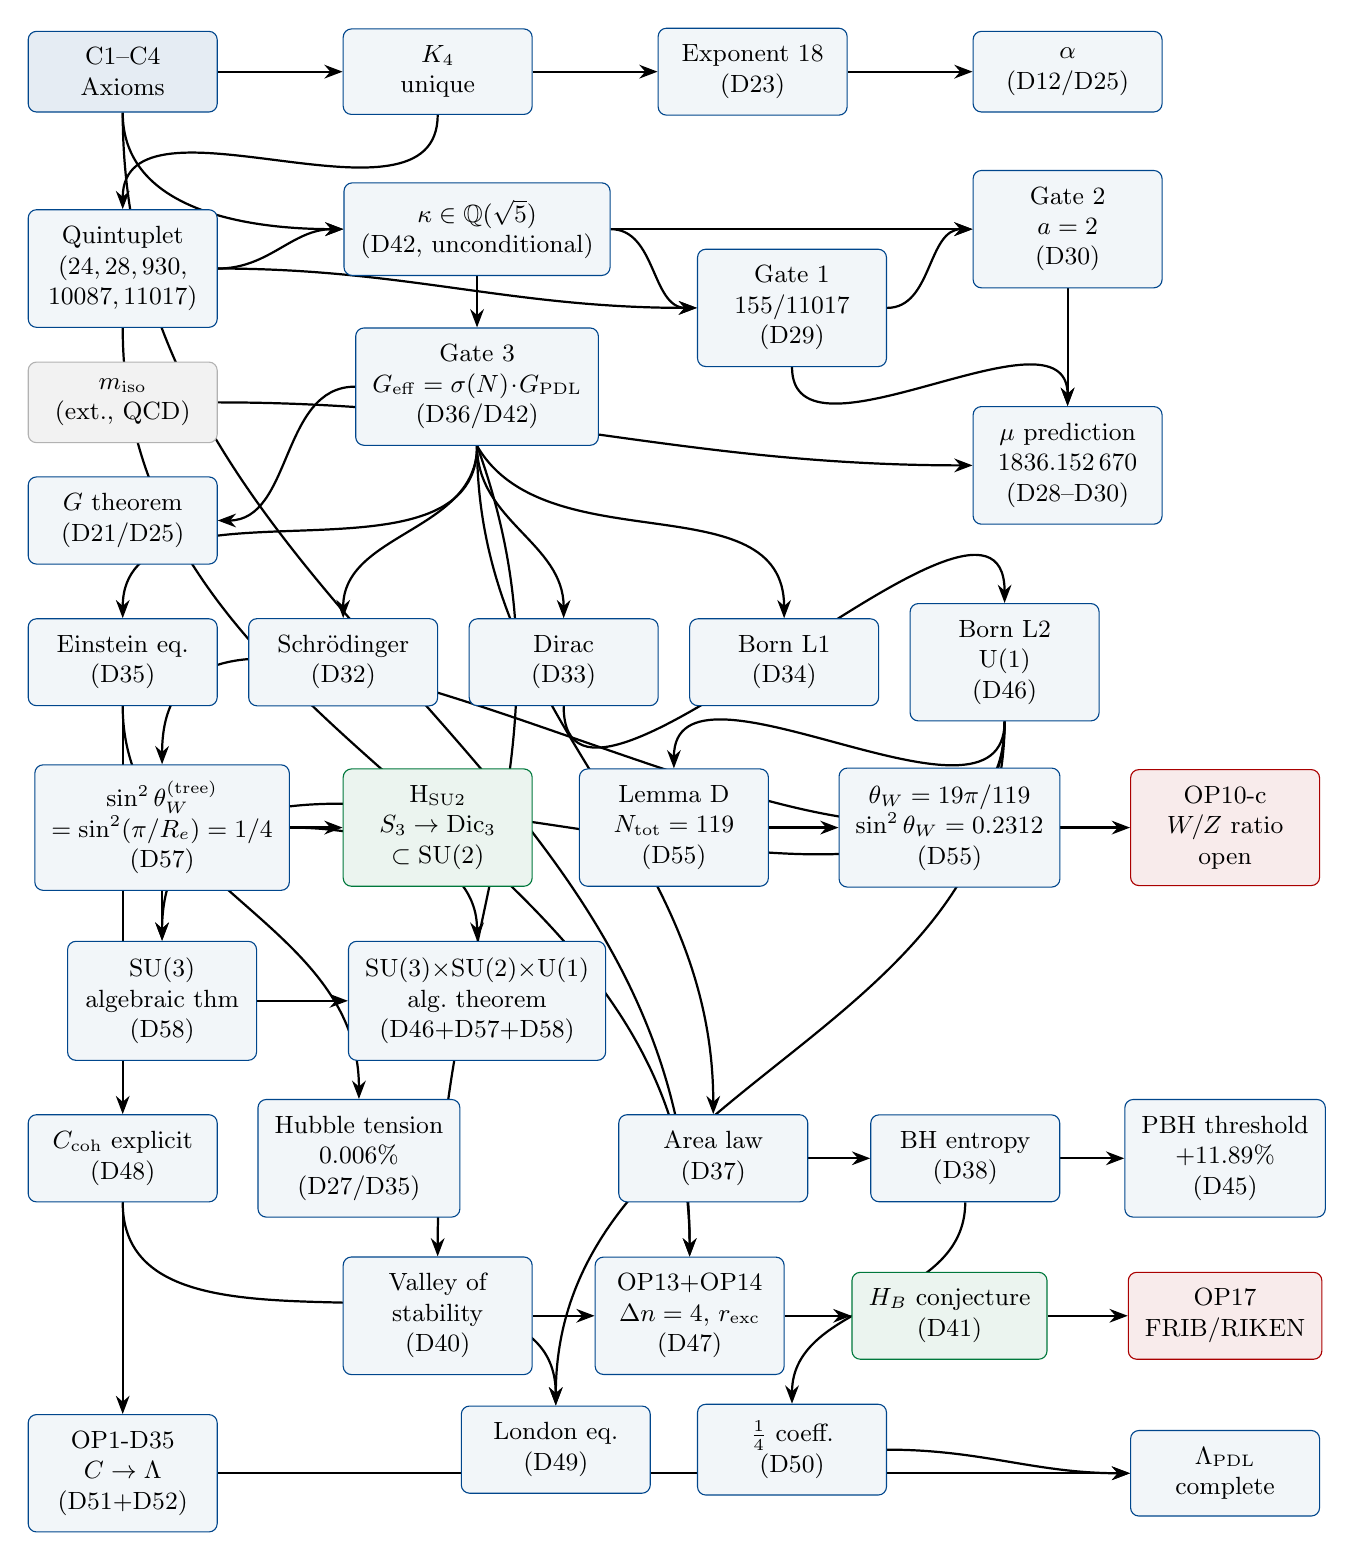
\begin{tikzpicture}[
  every node/.style={font=\small},
  axiom/.style={draw=proofblue, fill=proofblue!10,
    rounded corners=3pt, align=center, inner sep=6pt,
    minimum width=2.4cm, minimum height=0.9cm},
  theorem/.style={draw=proofblue, fill=proofblue!5,
    rounded corners=3pt, align=center, inner sep=6pt,
    minimum width=2.4cm, minimum height=0.9cm},
  conjecture/.style={draw=conjecturegreen, fill=conjecturegreen!8,
    rounded corners=3pt, align=center, inner sep=6pt,
    minimum width=2.4cm, minimum height=0.9cm},
  open/.style={draw=openproblemred, fill=openproblemred!8,
    rounded corners=3pt, align=center, inner sep=6pt,
    minimum width=2.4cm, minimum height=0.9cm},
  ext/.style={draw=gray!60, fill=gray!10,
    rounded corners=3pt, align=center, inner sep=6pt,
    minimum width=2.4cm, minimum height=0.9cm},
  arr/.style={-Stealth, thick},
]

% ── ROW 0 ── Axioms → K4 → Exp18 → alpha
\node[axiom]   at ( 0.0,  0.0) (C1C4)      {C1--C4\\Axioms};
\node[theorem] at ( 4.0,  0.0) (K4)        {$K_4$\\unique};
\node[theorem] at ( 8.0,  0.0) (exp18)     {Exponent~18\\(D23)};
\node[theorem] at (12.0,  0.0) (alpha)     {$\alpha$\\(D12/D25)};

% ── ROW 1 ── Quintuplet + kappa
\node[theorem] at ( 0.0, -2.5) (quintuplet){Quintuplet\\$(24,28,930,$\\$10087,11017)$};
\node[theorem] at ( 4.5, -2.0) (kappa)     {$\kappa\in\mathbb{Q}(\sqrt{5})$\\(D42, unconditional)};

% ── ROW 2 ── Gate1 + Gate2
\node[theorem] at ( 8.5, -3.0) (Gate1)     {Gate~1\\$155/11017$\\(D29)};
\node[theorem] at (12.0, -2.0) (Gate2)     {Gate~2\\$a=2$\\(D30)};

% ── ROW 3 ── miso + G + Gate3 + mu
\node[ext]     at ( 0.0, -4.2) (miso)      {$m_{\mathrm{iso}}$\\(ext., QCD)};
\node[theorem] at ( 0.0, -5.7) (G)         {$G$ theorem\\(D21/D25)};
\node[theorem] at ( 4.5, -4.0) (Gate3)     {Gate~3\\$G_{\mathrm{eff}}=\sigma(N)\!\cdot\!G_{\mathrm{PDL}}$\\(D36/D42)};
\node[theorem] at (12.0, -5.0) (mu)        {$\mu$ prediction\\$1836.152\,670$\\(D28--D30)};

% ── ROW 4 ── Einstein + Schrod + Dirac + Born L1 + Born L2
\node[theorem] at ( 0.0,-7.5) (Einstein)  {Einstein eq.\\(D35)};
\node[theorem] at ( 2.8,-7.5) (Schrod)    {Schr\"odinger\\(D32)};
\node[theorem] at ( 5.6,-7.5) (Dirac)     {Dirac\\(D33)};
\node[theorem] at ( 8.4,-7.5) (BornL1)    {Born L1\\(D34)};
\node[theorem] at (11.2,-7.5) (BornL2)   {Born L2\\U(1)\\(D46)};

 % ── ROW 4b ── Electroweak: k2 + LemmaD + Weinberg (D55) + D57 + WZ open
\node[theorem] at ( 0.5,-9.6) (D57tree)  {$\sin^2\theta_W^{(\mathrm{tree})}$\\$=\sin^2(\pi/R_e)=1/4$\\(D57)};
\node[conjecture] at ( 4.0,-9.6) (HSU2)  {H$_{\mathrm{SU2}}$\\$S_3\to\mathrm{Dic}_3$\\$\subset\mathrm{SU}(2)$};
\node[theorem] at ( 7.0,-9.6) (LemmaD)   {Lemma~D\\$N_{\mathrm{tot}}=119$\\(D55)};
\node[theorem] at (10.5,-9.6) (D55node)  {$\theta_W=19\pi/119$\\$\sin^2\theta_W=0.2312$\\(D55)};
\node[open]    at (14.0,-9.6) (WZopen)   {OP10-c\\$W/Z$ ratio\\open};

% ── D58 + SM gauge group
\node[theorem] at ( 0.5,-11.8) (D58node)  {$\mathrm{SU}(3)$\\algebraic thm\\(D58)};
\node[theorem] at ( 4.5,-11.8) (SMgauge)  {$\mathrm{SU}(3){\times}\mathrm{SU}(2){\times}\mathrm{U}(1)$\\alg.\ theorem\\(D46+D57+D58)};

% ── ROW 5 ── Ccoh + Hubble + AreaLaw + BH
\node[theorem] at ( 0.0,-13.8) (Ccoh)     {$\Ccoh$ explicit\\(D48)};
\node[theorem] at ( 3.0,-13.8) (Hubble)   {Hubble tension\\$0.006\%$\\(D27/D35)};
\node[theorem] at ( 7.5,-13.8) (AreaLaw)  {Area law\\(D37)};
\node[theorem] at ( 10.7,-13.8) (BH)       {BH entropy\\(D38)};
\node[theorem] at (14.0,-13.8) (D45)      {PBH threshold\\$+11.89\%$\\(D45)};

% ── ROW 6 ── Nuclear + D47 + HB + OP17
\node[theorem]    at ( 4.0,-15.8) (Nuclear) {Valley of\\stability\\(D40)};
\node[theorem]    at ( 7.2,-15.8) (D47node) {OP13+OP14\\$\Delta n=4$, $r_{\mathrm{exc}}$\\(D47)};
\node[conjecture] at ( 10.5,-15.8) (HB)      {$H_B$ conjecture\\(D41)};
\node[open]       at (14.0,-15.8) (OP17)    {OP17\\FRIB/RIKEN};

% ── ROW 7 ── D49 + D50 + D51/D52 + Lambda
\node[theorem] at ( 0.0,-17.8) (D51D52)  {OP1-D35\\$C\to\Lambda$\\(D51+D52)};
\node[theorem] at ( 5.5,-17.5) (D49)     {London eq.\\(D49)};
\node[theorem] at ( 8.5,-17.5) (D50)     {$\tfrac{1}{4}$ coeff.\\(D50)};
\node[theorem] at (14.0,-17.8) (Lambda)  {$\Lambda_{\mathrm{PDL}}$\\complete};

%% ══════════════════ FLÈCHES ══════════════════

\begin{pgfonlayer}{background}

% Row 0
\draw[arr] (C1C4.east)       -- (K4.west);
\draw[arr] (K4.east)         -- (exp18.west);
\draw[arr] (exp18.east)      -- (alpha.west);

% K4 → Quintuplet
\draw[arr] (K4.south)        to[out=-90, in=90] (quintuplet.north);

% Quintuplet + C1C4 → kappa
\draw[arr] (quintuplet.east) to[out=0, in=180] (kappa.west);
\draw[arr] (C1C4.south)      to[out=-90, in=180] (kappa.west);

% kappa + Quintuplet → Gate1
\draw[arr] (kappa.east)      to[out=0, in=180] (Gate1.west);
\draw[arr] (quintuplet.east) to[out=0, in=180] (Gate1.west);

% Gate1 → Gate2, kappa → Gate2
\draw[arr] (Gate1.east)      to[out=0, in=180] (Gate2.west);
\draw[arr] (kappa.east)      to[out=0, in=180] (Gate2.west);

% kappa → Gate3
\draw[arr] (kappa.south)     -- (Gate3.north);

% Gate3 → G
\draw[arr] (Gate3.west)      to[out=180, in=0] (G.east);

% Gate1 + Gate2 + miso → mu
\draw[arr] (Gate1.south)     to[out=-90, in=90]  (mu.north);
\draw[arr] (Gate2.south)     to[out=-90, in=90]  (mu.north);
\draw[arr] (miso.east)       to[out=0,   in=180] (mu.west);

% Gate3 → dynamics (row 4)
\draw[arr] (Gate3.south)     to[out=-90, in=90] (Einstein.north);
\draw[arr] (Gate3.south)     to[out=-90, in=90] (Schrod.north);
\draw[arr] (Gate3.south)     to[out=-90, in=90] (Dirac.north);
\draw[arr] (Gate3.south)     to[out=-60, in=90] (BornL1.north);
\draw[arr] (Dirac.south)     to[out=-90, in=90] (BornL2.north);

% Electroweak chain (D55)
\draw[arr] (BornL2.south)    to[out=-90, in=90] (D57tree.north);
\draw[arr] (D57tree.east)    -- (HSU2.west);
\draw[arr] (BornL2.south)    to[out=-90, in=90] (LemmaD.north);
\draw[arr] (LemmaD.east)     -- (D55node.west);
\draw[arr] (D55node.east)    -- (WZopen.west);

% D57 + D46 + D58 → SM gauge group
\draw[arr] (D57tree.south)   to[out=-90, in=90] (D58node.north);
\draw[arr] (BornL2.south)    to[out=-90, in=90] (D58node.north);
\draw[arr] (D58node.east)    -- (SMgauge.west);
\draw[arr] (D57tree.east)    to[out=0, in=90]   (SMgauge.north);

% Einstein → Ccoh, Hubble
\draw[arr] (Einstein.south)  -- (Ccoh.north);
\draw[arr] (Einstein.south)  to[out=-90, in=90] (Hubble.north);

% Ccoh → D49 (London), D51D52 (Lambda)
\draw[arr] (Ccoh.south)      -- (D51D52.north);
\draw[arr] (Ccoh.south)      to[out=-90, in=90] (D49.north);
\draw[arr] (BornL2.south)    to[out=-90, in=90] (D49.north);

% Gate3 → AreaLaw
\draw[arr] (Gate3.south)     to[out=-90, in=90] (AreaLaw.north);

% AreaLaw → BH
\draw[arr] (AreaLaw.east)    -- (BH.west);

% BH → D45, D50
\draw[arr] (BH.east)         -- (D45.west);
\draw[arr] (BH.south)        to[out=-90, in=90] (D50.north);

% Gate3 → Nuclear
\draw[arr] (Gate3.south)     to[out=-70, in=90] (Nuclear.north);

% Quintuplet + C1C4 → D47
\draw[arr] (quintuplet.south) to[out=-90, in=90] (D47node.north);
\draw[arr] (C1C4.south)       to[out=-90, in=90] (D47node.north);

% Nuclear + D47 → HB
\draw[arr] (Nuclear.east)    -- (D47node.west);
\draw[arr] (D47node.east)    -- (HB.west);

% D51D52 + D50 → Lambda
\draw[arr] (D51D52.east)     to[out=0, in=180] (Lambda.west);
\draw[arr] (D50.east)        to[out=0, in=180] (Lambda.west);

% HB → OP17
\draw[arr] (HB.east)         -- (OP17.west);

\end{pgfonlayer}

\end{tikzpicture}%
}
\caption{Critical-path dependency map of the PDL programme (v23). \textcolor{proofblue}{Blue nodes}: unconditional theorems. \textcolor{conjecturegreen}{Green}: conjectures. \textcolor{openproblemred}{Red}: open problems. Grey: unique external input ($m_{\mathrm{iso}}$). The quantum dynamics layer (Schr\"odinger, Dirac, Born L1, Born L2/U(1), London equation), the nuclear stability layer (OP13, OP14, valley of stability), the black hole thermodynamics layer (area law, Bekenstein--Hawking, $\tfrac{1}{4}$ coefficient), the cosmological leakage layer ($C \to \Lambda_{\mathrm{PDL}}$), and the electroweak sector ($\theta_W = 19\pi/119$, D55) are all complete theorems of C1--C4. The causal chain C1--C4 $\to$ $\Lambda_{\mathrm{PDL}}$ is fully closed; the electroweak gauge geometry is structurally derived. The algebraic structure $\mathrm{SU}(3)\times\mathrm{SU}(2)\times\mathrm{U}(1)$ of the Standard Model gauge group is now an unconditional theorem of C1--C4 (D46+D57+D58). Remaining open: physical identification of $\mathrm{SU}(3)_c$ (OP-D58-1), $W/Z$ mass ratio (OP10-c), and experimental lattice QCD test of $\Delta m_{\mathrm{iso}}$ (OP10-d).}
\label{fig:dependency}
\end{figure}

\newpage

% ============================================================
\section{Falsifiable Predictions}
\label{sec:predictions}

\begin{longtable}{L{0.5cm}L{3.2cm}L{5.2cm}L{4.2cm}}
\caption{Complete list of falsifiable, parameter-free PDL predictions (v20). All predictions follow from the quintuplet and $m_{\mathrm{iso}}$ alone, with no additional free parameters. Predictions P1--P6 are derived from the analytical chain; P7--P8 follow from Conjecture~$H_B$ (D41); P9 is derived from D45.}
\label{tab:predictions}\\
\toprule
\textbf{ID} & \textbf{Observable} & \textbf{PDL prediction} & \textbf{Test / status}\\
\midrule
\endfirsthead
\toprule
\textbf{ID} & \textbf{Observable} & \textbf{PDL prediction} & \textbf{Test / status}\\
\midrule
\endhead
\bottomrule
\endfoot
P1 & Proton--electron mass ratio $\mu$ & $\mu=1836.152\,670$ (parameter-free) & Testable at $0.001$~ppm; current CODATA: $1836.152\,673\,43(11)$; residual $1.8\times10^{-9}$.\\[0.4em]
P2 & Fine-structure constant $\alpha$ & $\alpha^{-1}=137.035\,999$ from quintuplet alone & Testable at $10^{-9}$; current agreement $\mathcal{O}(10^{-4})$; OP3/OP7 for residual.\\[0.4em]
P3 & Hubble constant ratio & $H_{0,\mathrm{local}}/H_{0,\mathrm{CMB}}=\sigma(N_{\mathrm{local}})/\sigma(40)$ & PDL prediction $1.085935$ vs.\ observed $1.0859\pm0.007$; $0.006\%$ error; zero free parameters.\\[0.4em]
P4 & CMB-epoch BH entropy suppression & Factor $\sigma(40)\approx 0.848$ relative to local universe & No direct observation yet; accessible via future CMB-$S_4$ constraints.\\[0.4em]
P5 & PBH survival threshold & $M^*_{\mathrm{PDL}}=\sigma(40)^{-2/3}\,M^*_{\mathrm{GR}}\approx 5.706\times10^{14}$\,g ($+11.89\%$) & Testable via Fermi-LAT IGRB analysis with \textsc{BlackHawk}/\textsc{Isatis}~\cite{D45}; excess Hawking flux at $\sim93$--$104$\,MeV.\\[0.4em]
P6 & AGN entropy-to-energy ratio & $S/E\propto G(N(z))$: systematic redshift trend & Traceable in cosmic-noon AGN surveys (JWST, Euclid); no contradicting data.\\[0.4em]
P7 & $B(E2)$ ratio in $^{90}$Ru/$^{88}$Ru & $R\approx 2.02$ (from $H_B$, $k=8\to10$) & Testable at FRIB or RIKEN; $^{88}$Ru beam available.\\[0.4em]
P8 & $N_{\mathrm{comp}}$ ratio $^{94}$Pd/$^{92}$Pd & $N_{\mathrm{comp}}(^{94}\mathrm{Pd})/N_{\mathrm{comp}}(^{92}\mathrm{Pd})=2.000\pm0.05$ & Testable from DNO-SM calculations with $^{94}$Pd spectroscopy at RIKEN.\\[0.4em]
P9 & IGRB spectral cutoff position & $E_c^{\mathrm{PDL}} \approx 93$\,MeV vs.\ $E_c^{\mathrm{GR}} \approx 104$\,MeV (shift $-10.6\%$) & Testable with Fermi-LAT IGRB data + \textsc{BlackHawk}/\textsc{Isatis}; requires non-zero $f_{\mathrm{PBH}}$ in $[5.10,\,5.71]\times10^{14}$\,g.\\[0.4em]
P10 & Isospin mass splitting $\Delta m_{\mathrm{iso}}$ & $\Delta m_{\mathrm{iso}} = 2.446$~MeV (from D55 C1+C3 formula, no free parameter) & FLAG 2024: $2.52 \pm 0.08$~MeV; compatible at $0.92\,\sigma$. Distinguishable from D30 value ($2.532$~MeV) at $\pm 0.04$~MeV precision (next-generation lattice QCD, 3--5 year horizon).\\[0.4em]
\end{longtable}

% ============================================================
\section{Continuation Guide}
\label{sec:continuation}

\subsection{Entry points}
\label{subsec:entrypoints}
The following entry points are recommended for a colleague wishing to contribute to specific open problems.

\begin{itemize}
\item \textbf{OP1-D35 (leak constant $C$):} The most significant remaining foundational problem. Requires familiarity with D48 (coherence tensor), D17 (exponent~18 derivation), and D30 ($\eta_L$ structural factor). The question is whether the prefactor $C$ in $C^{(\mathrm{leak})}$ can be expressed as a closed-form function of the quintuplet, in the spirit of OP-B (resolved in D44).
\item \textbf{OP2 (global uniqueness):} Requires familiarity with D16, D16b, and combinatorial optimisation over integer lattices. The Colab infrastructure of D43 can be used to extend the computational search radius.
\item \textbf{OP7 (47~ppm residual in $\mu$):} Immediately actionable using the D43 Colab infrastructure. Start with the Group~I filters in D43, identify the residual at each stage, and test candidate combinatorial factors from C1--C4.
\item \textbf{OP12 (BH coefficient $\tfrac{1}{4}$):} \textcolor{proofblue}{Resolved by D50.} The coefficient $\tfrac{1}{4}$ in $\SBH = k_B A/(4\ell_P^2)$ is the stable fraction $4/16$ per surface relation (D29), with independence guaranteed by H3 (D42). $\Omega_{\mathrm{surf}} = 4^{\Rsurf}$, $S_{\mathrm{surf}} = k_B\Rsurf\ln 4$. Black hole thermodynamics layer complete.
\item \textbf{OP-London (London equation from PDL):} \textcolor{proofblue}{Resolved by D49.} See corpus table entry above.
\item \textbf{OP1-D35 (leak constant $C$):} \textcolor{proofblue}{Resolved by D51+D52.} See corpus table entry and Section~\ref{sec:openproblems} above.
\end{itemize}

\subsection{Recommended next documents}
\label{subsec:nextdocs}
Given the current state of the programme, the following documents would have the highest impact:

\begin{enumerate}
\item \textbf{DM v26}: The present document. Incorporates D58 ($\mathrm{SU}(3)$ as unconditional algebraic theorem, completion of $\mathrm{SU}(3)\times\mathrm{SU}(2)\times\mathrm{U}(1)$) and its supplementary script \texttt{PDL\_SU3\_script1.py}.
\item \textbf{D59 --- Physical identification of $\mathrm{SU}(3)_c$}: Construct the fundamental representation $\mathbf{3}$ of $\mathrm{SU}(3)$ as an action on a PDL triplet; identify with the colour gauge group. Requires Colab verification before drafting. \textbf{Entry point:} D47, D51, D52, D58 (OP-D58-1).
\item \textbf{OP-D57-1 --- Lemma C1-$V_4$}: Proving formally that C1 forces $V_4$ trivial would promote H$_{\mathrm{SU2}}$ to a theorem. \textbf{Entry point:} D46, D57.
\item \textbf{OP-E2-PDL}: Identification of the $E2$ operator in the PDL formalism (D29, D32, D41, D56). Resolving this would elevate Conjecture~$H_B$ to a theorem.
\item \textbf{D-electroweak-WZ}: Derivation of the $W/Z$ mass ratio $M_W/M_Z = \cos(19\pi/119)$ as a parameter-free prediction (OP10-c). Entry point: D55, D57.
\item \textbf{Experimental confrontations}: (i) FLAG/lattice QCD for $\Delta m_{\mathrm{iso}}$ at $\pm 0.04$~MeV (D55, P10). (ii) D45 predictions to \textsc{BlackHawk}/\textsc{Isatis} community, Fermi-LAT IGRB 50--200\,MeV window.
\item \textbf{D-nuclear-Z>82}: Extension of the valley-of-stability theorem to $Z>82$ (OP15).
\item \textbf{DL03}: Numerical enclosure of $n^*_{\mathrm{life}}$ from the gain function $R^1_{\mathrm{active}}$.
\end{enumerate}


% ============================================================
\section{Glossary}
\label{sec:glossary}

\begin{description}[leftmargin=3.5cm, style=nextline]
\item[AB criterion] The two-part stability criterion (amplitude condition A + balance condition B) that selects admissible two-closure couplings; proved exhaustively in D29 over $768$ configurations.
\item[Active surface $\Rsurf$] The set of valence coherence relations of the proton, $|\Rsurf|=\sigma=930$; the locus of all physical information exchange.
\item[Admissible closure] A finite signed graph satisfying all four axioms C1--C4; the minimal example is $K_4$.
\item[Born Level~1 / Level~2] Level~1 (D34, Theorem): modulus rule $P=|\psi|^2$ proved via Gleason uniqueness. Level~2 (D46, Theorem, OP4 resolved): $\mathrm{U}(1)$ phase freedom derived from $K_4$ sign equivalence and Hopf fibration structure.
\item[$\Ccoh$] Coherence stress-energy tensor appearing in the PDL Einstein equation; explicit form derived in D48v3, D51, D52: $C^{(\mathrm{mass})}$, $C^{(\mathrm{orb})}$, $C^{(\mathrm{spin})}$, and $C^{(\mathrm{leak})}$ all unconditional theorems. $C^{(\mathrm{spin})}=0$ in the ground state (OP-spin resolved, D48v3). All components in uniform units J\,m$^{-3}$. OP2-D35, OP1-D35, and OP-spin fully resolved.
\item[Coherence cost] Fraction of violated triangles (negative-product edges) in a signed graph; minimised by axiom C4.
\item[DL series] Documents DL01, DL02, \ldots; the PDL-V programme extending C1--C4 to self-replication and complexity thresholds. Structurally separate from the D series; presented in Part~III of this document.
\item[$\delta^*$] Optimal lineage variation in the PDL-V programme; $\delta^* = 1/2$, equal to the half-pulsation of $K_4$; proved invariant under the rarity law (DL01).
\item[$\epsGeomB$] Geometric correction factor in the PDL mass-ratio formula; closed-form expression $\epsGeomB = \kappa \cdot C/(6+\kappa)\cdot(1+2/\Rtot) \in \mathbb{Q}(\sqrt{5})$ proved in D44 (OP8 resolved).
\item[Equation of state $w(N)$] The ratio $P/(\rhocoh c^2)$ for the PDL coherence fluid; $w(N) = -\rho_\Lambda/\rhocoh(N)$ (D54, unconditional theorem). At coherence densities $|w| \sim 10^{-44}$ (cold matter); at cosmological scales $\Omega_\Lambda^{\mathrm{PDL}} = 0.6838$ (dark energy, $0.17\%$ from Planck 2020).
\item[$f(n)$] Rarity law in the PDL-V programme; $f(n) = 2^{n+1-\binom{n}{2}}$, doubly exponentially decreasing; exponents are triangular numbers (DL01, exact theorem).
\item[$\Geff(N)$] Effective gravitational coupling at scale $N$; equal to $\sigmaN\cdot\GPDL$ by Gate~3 (unconditional theorem).
\item[Gate 1, 2, 3] Three critical proof milestones. Gate~1: $155/11017$ from axioms (D29). Gate~2: $a=2$ from axioms (D30). Gate~3: $\Geff=\sigmaN\cdot\GPDL$ (D36/D42, unconditional).
\item[H1, H2, H3] Named hypotheses of the programme. H1 ($\kappa=\sigma/R_{\mathrm{tot}}$): now an unconditional theorem (follows from H3/D42 via D39). H2 (bridge linearity): absorbed into D36. H3 (Indifference Lemma): proved unconditionally in D42.
\item[Hopf fibration] The fibre bundle $S^1\hookrightarrow S^3\to S^2$ generating the $\mathrm{U}(1)$ phase freedom of quantum mechanics; its appearance in D46 is a structural consequence of the $K_4$ pulsation sign equivalence.
\item[Indifference Lemma (H3)] The probability measure on the relations of a PDL closure is uniform; the unique measure compatible with $S_4$-symmetry of $K_4$. Proved from C1--C4 in D42 via three lemmas.
\item[$K_4$] The complete signed graph on four vertices and six edges; the unique minimal admissible closure (D16a theorem); identified with the electron prototype.
\item[$\kappa$] Primary leakage parameter; $\kappa=310\varphi/11017\in\mathbb{Q}(\sqrt{5})$; unconditional theorem of C1--C4 (D42 corollary); $\kappa\approx 0.0455$.
\item[Mirror Lemma] The proton and neutron HO-PDL levels are isomorphic, sharing the same splitting $s=1/12$, level order, and degeneracies (D47, Lemma~5.2, from D22-N2).
\item[$m_{\mathrm{iso}}$] Isospin mass splitting $m_d-m_u$; the unique irreducible external parameter of the programme (Gate~2, D30).
\item[$N_{\mathrm{CMB}}$] PDL-derived CMB epoch parameter; $N_{\mathrm{CMB}}=40$ from neutron quintuplet (D27 theorem).
\item[$n^*_{\mathrm{life}}$, $n^*_{\mathrm{consciousness}}$, $n^*_{\mathrm{max}}$] Life, consciousness, and maximum complexity thresholds in the PDL-V programme; existence and strict ordering proved (DL02); numerical values open (DL-OP1, DL-OP2).
\item[OP$n$] Open Problem $n$; see Section~\ref{sec:openproblems}. OP1, OP4, OP8, OP12, OP13, OP14, OP-London, OP1-D35, and OP-pressure fully resolved.
\item[PDL] Projective Dynamic Logo; the research programme initiated in D01.
\item[PDL-V programme] Extension of PDL to self-replication and complexity thresholds; inaugurated by DL01 and DL02; see Part~III.
\item[Quintuplet] The integer tuple $\quintuplet$ characterising the proton; $\nu_u=24$, $\nu_d=28$, $\sigma=930$, $R_{\mathrm{sea}}=10087$, $R_{\mathrm{tot}}=11017$.
\item[$\rhocoh(N)$] Coherence mass density at scale $N$; $\rhocoh = \sigmaN\cdot\Rsurf\cdot m_p/(V_C\cdot\Rtot)$ (D48v3 theorem).
\item[$S(\Gamma)$] Constraint-structure operator in the PDL-V programme; $S(K_4) \cong K_4$ (DL01 theorem).
\item[$\sigmaN(N)$] Coherence engagement fraction at scale $N$; $\sigmaN=1-(1-\kappa)^N\in\mathbb{Q}(\sqrt{5})$; $\sigmaN(40)\approx 0.8449$.
\item[$\Tpp$] Proton--proton conflict unit; $C(Z>20)=190\,\Tpp$ exactly (D40 theorem).
\item[$V_C$] Coherence volume; $V_C=(4/3)\pi[\hbar/(m_pc)]^3$; unconditional theorem of C1--C4 via D10a (temporal chain, Chain~1). D48v3 theorem.
\item[Valley of stability] Minimum neutron number $N_{\min}(Z)$ for stable nuclei; reproduced at $100\%$ accuracy for $Z=1$--82 as an unconditional theorem of C1--C4 (D40, D47 corollary).
\item[18-filter hierarchy] The decomposition $18=6+5+4+3$ of the leakage exponent into four topological levels (D06, D17, D23).
\end{description}

% ============================================================
\newpage
\part{The PDL-V Programme: Life and Consciousness}
\label{part:PDL-V}
% ============================================================

\begin{center}
\textit{This Part is structurally separate from Parts I and II.\\
It presents a rigorous extension of the PDL framework to self-replication\\
and complexity thresholds, in a domain distinct from the physical constants programme.\\
The same axioms C1--C4 are used; the domain of application is different.}
\end{center}

\vspace{1em}

% ============================================================
\section{Introduction to the PDL-V Programme}
\label{sec:PDLV_intro}
% ============================================================

The PDL-V programme asks whether the axioms C1--C4, which determine the proton architecture and all derived physical constants, also constrain the structural conditions for self-replication and the emergence of biological and cognitive complexity. Documents DL01 and DL02 do not make biological claims; they establish mathematical threshold theorems that any system satisfying C1--C4 must obey. The connection to biology and consciousness is conjectural and is explicitly labelled as such.

\subsection{Separation from the physics programme}

The DL series shares the axiomatic foundation (C1--C4 and $K_4$) with the D series, but operates in a domain where the ``configurations'' are hierarchical graph structures rather than physical coherence cycles. The results of DL01 and DL02 are theorems of C1--C4 applied to this domain, with full epistemic rigour, but their physical interpretation involves a conjecture (the PDL-V Conjecture, DL01) that is not yet derivable from first principles. This conjecture is explicitly identified and is not presented as a theorem.

\subsection{Reading note}

A reader whose sole interest is the physical constants programme (gravitational constant, cosmological constant, nuclear structure, etc.) may skip Part~III without loss of continuity. A reader interested in the structural limits of self-replication and complexity should read DL01 first (operators $L$, $S$, $R^k$; rarity law; $\delta^*$ invariant), then DL02 (threshold hierarchy theorem).

% ============================================================
\section{Self-Replication Operators and the Rarity Law (DL01)}
\label{sec:DL01}
% ============================================================

\begin{theorem}[$K_4$ fixed point of $S$, \cite{DL01}]
\label{thm:DL01_fixedpoint}
Let $S(\Gamma)$ be the constraint-structure operator acting on admissible signed graphs. The complete graph $K_4$ is the unique fixed point of $S$: $S(K_4) \cong K_4$. This has been verified computationally over all 8 coherent configurations of $K_4$.
\end{theorem}

\begin{theorem}[Rarity law and $\delta^*$ invariant, \cite{DL01}]
\label{thm:DL01_rarity}
The fraction of self-replicating configurations at level $n$ satisfies the exact law:
\begin{equation}
f(n) = 2^{n+1-\binom{n}{2}},
\end{equation}
with exponents equal to $-T_{n-2}$ (triangular numbers): $f(n)$ is doubly exponentially decreasing. The optimal lineage variation $\delta^* = 1/2$ is an invariant equal to the half-pulsation of $K_4$; it is independent of $n$. The weak self-representation relation $R^1_{\mathrm{weak}}$ is forced at $100\%$ for all $n \geq 4$, verified for $n = 4$--$7$.
\end{theorem}

% ============================================================
\section{Threshold Hierarchy Theorems (DL02)}
\label{sec:DL02}
% ============================================================

\begin{theorem}[$K_4$ unique fixed point, \cite{DL02}]
\label{thm:DL02_unique}
$K_4$ is the unique fixed point of $S$ over all admissible closures. The equation $C(n,3) = n(n-1)(n-2)/6 = 4$ has $(n-1)(n-2) = 6$ as its only positive integer solution: $n = 4$. This is an unconditional theorem of C1--C4.
\end{theorem}

\begin{theorem}[Strict threshold separation, \cite{DL02}]
\label{thm:DL02_separation}
For $n \geq 5$, $|S^1(K_n)| \neq |S^2(K_n)|$: the first and second iteration of $S$ produce distinct orbit sizes. This forces a strict separation between the life threshold and the consciousness threshold: $n^*_{\mathrm{life}} < n^*_{\mathrm{consciousness}}$. This is an unconditional theorem of C1--C4.
\end{theorem}

\begin{theorem}[Finiteness of all thresholds, \cite{DL02}]
\label{thm:DL02_finiteness}
The doubly exponential rarity law $f(n) = 2^{n+1-\binom{n}{2}}$ implies that all thresholds $n^*$ are finite: $n^*_{\mathrm{max}} < \infty$. Combined with Theorems~\ref{thm:DL02_unique} and~\ref{thm:DL02_separation}, this gives the unconditional hierarchy:
\begin{equation}
4 \;<\; n^*_{\mathrm{life}} \;<\; n^*_{\mathrm{consciousness}} \;<\; n^*_{\mathrm{max}} \;<\; \infty.
\end{equation}
\end{theorem}

\subsection{Open problems in the PDL-V programme}

\begin{openproblem}[DL-OP1 --- Numerical value of $n^*_{\mathrm{life}}$]
\label{op:DL_nlife}
The existence and strict ordering of $n^*_{\mathrm{life}}$ is established analytically (DL02). Its numerical value remains open. The gain function $R^1_{\mathrm{active}}(n)$ must be derived in closed form and its first zero located. \textbf{Priority:} high. \textbf{Entry point:} DL01, DL02.
\end{openproblem}

\begin{openproblem}[DL-OP2 --- Numerical value of $n^*_{\mathrm{consciousness}}$]
\label{op:DL_nconsciousness}
Analogous to DL-OP1 but for the second threshold. Requires DL-OP1 as a prerequisite. \textbf{Priority:} medium. \textbf{Entry point:} DL01, DL02.
\end{openproblem}

\begin{openproblem}[DL-OP3 --- Connection to physical substrate]
\label{op:DL_substrate}
The PDL-V conjecture (DL01) proposes that the threshold $n^*_{\mathrm{life}}$ corresponds to a specific physical structure derivable from C1--C4. This connection has not been derived and remains a conjecture. A formal derivation would require identifying the physical interpretation of the graph complexity level $n$ in terms of molecular or cellular organisation. \textbf{Priority:} exploratory. \textbf{Entry point:} DL01.
\end{openproblem}

\clearpage

% ============================================================
\bibliographystyle{unsrturl}
\bibliography{DM_v26_references}

\end{document}